\subsection{CONTINUITY AND DIFFERENTIABILITY OF CONVEX FUNCTIONS}

PROPOSITION 5. For a real finite function f to be convex (resp. strictly convex) on an interval I it is necessary and sufficient that for all \(a \in I\) the gradient

\[
p (\mathbf {M} _ {a} \mathbf {M} _ {x}) = \frac {f (x) - f (a)}{x - a}
\]

be an increasing (resp. strictly increasing) function of x on I ∩ ∁\{a\}.

This proposition is an immediate consequence of definitions 1 and 2 and of the lemma of I, p.~23.

PROPOSITION 6. Let \(f\) be a finite real function convex on an interval \(\mathbf{I} \subset \mathbf{R}\) . Then at every interior point \(a\) of \(\mathbf{I}\) the function \(f\) is continuous, has finite right and left derivatives, and \(f_g'(a) \leqslant f_d'(a)\) .

Indeed, for \(x \in I\) and \(x > a\) the function \(x \mapsto \frac{f(x) - f(a)}{x - a}\) is increasing (prop. 5) and bounded below, since if \(y < a\) and \(y \in I\) we have

\[
\frac {f (y) - f (a)}{y - a} \leqslant \frac {f (x) - f (a)}{x - a}\tag{5}
\]

by prop. 5; this function therefore has a finite right limit at the point \(a\) ; in other words, \(f_d'(a)\) exists and is finite; further, letting \(x\) approach \(a\) ( \(x > a\) ) in (5), it follows that

\[
\frac {f (y) - f (a)}{y - a} \leqslant f _ {d} ^ {\prime} (a)\tag{6}
\]

for all \(y < a\) belonging to I. In the same way one shows that \(f_{g}^{\prime}(a)\) exists and that

\[
f _ {d} ^ {\prime} (a) \leqslant \frac {f (x) - f (a)}{x - a}\tag{7}
\]

for \(x \in I\) and x \textgreater{} a. On letting x approach \(a (x > a)\) in this last inequality we obtain \(f_{g}^{\prime}(a) \leqslant f_{d}^{\prime}(a)\) . The existence of the left and right derivatives at the point a clearly ensures the continuity of f at this point.

COROLLARY 1. Let \(f\) be a convex (resp. strictly convex) function on I; if \(a\) and \(b\) are two interior points of I such that \(a < b\) one has (fig.~3)

\pandocbounded{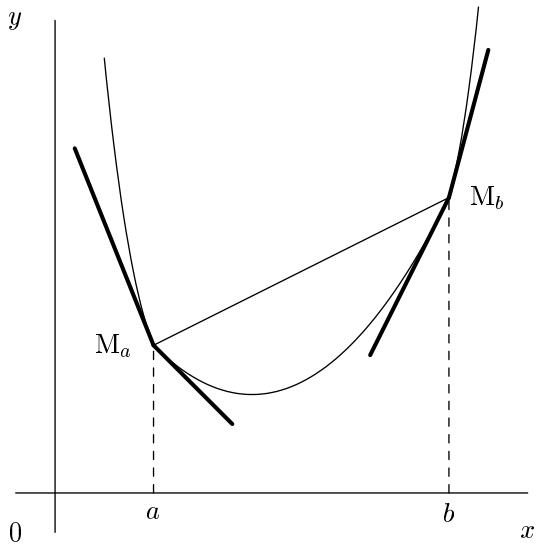
\includegraphics[keepaspectratio]{images/part001_a227d9e4.jpg}}\\
Fig. 3

\[
f _ {d} ^ {\prime} (a) \leqslant \frac {f (b) - f (a)}{b - a} \leqslant f _ {g} ^ {\prime} (b)\tag{8}
\]

(resp.

\[
f _ {d} ^ {\prime} (a) <   \frac {f (b) - f (a)}{b - a} <   f _ {g} ^ {\prime} (b)).\tag{9}
\]

The double inequality (8) results from (6) and (7) by a simple change of notation. On the other hand, if \(f\) is strictly convex and \(c\) is such that \(a < c < b\) one has, from (8) and prop. 5,

\[
f _ {d} ^ {\prime} (a) \leqslant \frac {f (c) - f (a)}{c - a} <   \frac {f (b) - f (a)}{b - a} <   \frac {f (b) - f (c)}{b - c} \leqslant f _ {g} ^ {\prime} (b)
\]

from which (9).

COROLLARY 2. If f is convex (resp. strictly convex) on I then \(f_{d}^{\prime}\) and \(f_{g}^{\prime}\) are increasing (resp. strictly increasing) on the interior of I; the set of points in I at which f is not differentiable is countable, and \(f_{d}^{\prime}\) and \(f_{g}^{\prime}\) are continuous at every point where f is differentiable.

The first part follows immediately from (8) (resp. (9)) and the inequality

\[
f _ {g} ^ {\prime} (a) \leqslant f _ {d} ^ {\prime} (a).
\]

On the other hand, let E be the set of interior points x of I where f is not differentiable (that is \(f_{g}^{\prime}(x) < f_{d}^{\prime}(x)\) ). For each \(x \in E\) let \(J_{x}\) be the open interval \(]f_{g}^{\prime}(x), f_{d}^{\prime}(x)[;\) it follows from (8) that if x and y are two points of E such that x \textless{} y, then u \textless{} v for all \(u \in J_{x}\) and all \(v \in J_{y}\) ; in other words, as x runs through E the open nonempty intervals \(J_{x}\) are pairwise disjoint; the set of such intervals is thus countable, and hence so is E. Finally, \(f_{d}^{\prime}\) (resp. \(f_{g}^{\prime}\) ) being increasing, it has a right limit and a left limit at every interior point x of I; prop. 6 of I, p.~18 now shows that the right limit of \(f_{d}^{\prime}\) (resp. \(f_{g}^{\prime}\) ) at the point x is equal to \(f_{d}^{\prime}(x)\) , and its left limit is \(f_{g}^{\prime}(x)\) ; from which we have the last part of the corollary.

Let \(f\) be a convex function on \(I, a\) an interior point of \(I\) , and \(D\) a line passing through the point \(M_a\) , with equation \(y - f(a) = \alpha(x - a)\) . It follows from the inequalities (8) that if \(f_g'(a) \leqslant \alpha \leqslant f_d'(a)\) then every point of the graph \(G\) lies above \(D\) , and, if \(f\) is strictly convex, \(M_a\) is the only point common to \(D\) and \(G\) ; one says that \(D\) is a support line to \(G\) at the point \(M_a\) . Conversely, if \(G\) lies above \(D\) , one has \(f(x) - f(a) \geqslant \alpha(x - a)\) for every \(x \in I\) , from which \(\frac{f(x) - f(a)}{x - a} \geqslant \alpha\) for \(x > a\) , and \(\frac{f(x) - f(a)}{x - a} \leqslant \alpha\) for \(x < a\) ; on letting \(x\) tend to \(a\) in these inequalities it follows that \(f_g'(a) \leqslant \alpha \leqslant f_d'(a)\) .

In particular, if \(f\) is differentiable at the point \(a\) there is only one supporting line to \(G\) at the point \(M_a\) , the tangent to \(G\) at \(M_a\) .

Remark. If \(f\) is a strictly convex function on an open interval \(I\) then \(f_d'\) is strictly increasing on \(I\) , so there are three possible cases, according to prop. 2 of \(I\) , p.~13:

\(1^{\circ} f\) is strictly decreasing on I;

\(2^{\circ}\) f is strictly increasing on I;

\(3^{\circ}\) there is an \(a \in \mathrm{I}\) such that \(f\) is strictly decreasing for \(x \leqslant a\) , and is strictly increasing for \(x \geqslant a\) .

When \(f\) is convex on \(I\) , but not strictly convex, \(f\) can be constant on an interval contained in \(I\) ; let \(J = ]a, b[\) be the largest open interval on which \(f\) is constant (that is to say, the interior of the interval where \(f_{d}^{\prime}(x)=0\)) ; then f is strictly decreasing on the interval formed by the points \(x\in I\) such that \(x\leqslant a\) (if it exists), strictly increasing on the interval formed by the points \(x\in I\) such that \(x\geqslant b\) (if it exists).

In all cases one sees that \(f\) possesses a right limit at the left-hand endpoint of I (in \(\overline{\mathbf{R}}\) ), and a left limit at the right-hand endpoint; these limits may be finite or infinite (cf.~I, p.~46, exerc. 5, 6 and 7). By abuse of language one sometimes says that the continuous function (with values in \(\overline{\mathbf{R}}\) ), equal to \(f\) on the interior of I, and extended by continuity to the endpoints of I, is convex on \(\overline{\mathbf{I}}\) .

\subsection{CRITERIA FOR CONVEXITY}

PROPOSITION 7. Let f be a finite real function defined on an interval \(I \subset R\) . For f to be convex on I it is necessary and sufficient that for every pair of numbers a, b of I such that a \textless{} b, and for every real number \(\mu\) , the function \(f(x) + \mu x\) attains its supremum on \([a, b]\) at one of the points a, b.

The condition is necessary; indeed, since \(\mu x\) is convex on \(\mathbf{R}\) , the function \(f(x) + \mu x\) is convex on I; one can therefore restrict oneself to the case \(\mu = 0\) . Then, for

\[
x = \lambda a + (1 - \lambda) b \quad (0 \leqslant \lambda \leqslant 1),
\]

one has

\[
f (x) \leqslant \lambda f (a) + (1 - \lambda) f (b) \leqslant \operatorname{Max} (f (a), f (b)).
\]

The condition is sufficient. Let us take \(\mu = -\frac{f(b) - f(a)}{b - a}\) and let \(g(x) = f(x) + \mu x\) ; one has \(g(a) = g(b)\) and therefore \(g(x) \leqslant g(a)\) for all \(x \in [a, b]\) , and one can check immediately that this inequality is equivalent to the inequality (1) where one replaces \(z\) by \(a\) and \(x'\) by \(b\) .

PROPOSITION 8. For a finite real function f to be convex (resp. strictly convex) on an open interval \(I \subset R\) it is necessary and sufficient that it be continuous on I, have a derivative at every point of the complement B relative to I of a countable subset of this interval, and that the derivative be increasing (resp. strictly increasing) on B.

The condition is necessary, from prop. 6 and its corollary 2 (I, p.~27); let us show that it is sufficient. Suppose, therefore, that \(f'\) is increasing on B, and that \(f\) is not convex; there then exist (I, p.~27, prop. 5) three points \(a, b, c\) of I, such that \(a < c < b\) , and \(\frac{f(c) - f(a)}{c - a} > \frac{f(b) - f(c)}{b - c}\) ; but from the mean value theorem (I, p.~14, th. 1) one has

\[
\frac {f (c) - f (a)}{c - a} \leqslant \sup _ {x \in \mathrm{B}, a <   x <   c} f ^ {\prime} (x) \quad \text { and } \quad \frac {f (b) - f (c)}{b - c} \geqslant \inf _ {x \in \mathrm{B}, c <   x <   b} f ^ {\prime} (x).
\]

One thus has \(\sup_{x\in \mathbf{B},a < x < c}f'(x) > \inf_{x\in \mathbf{B},c < x < b}f'(x)\) , contrary to the hypothesis that \(f'\) is increasing on B.

If now we assume that \(f'\) is strictly increasing on B, then \(f\) is convex and cannot be equal to an affine linear function on any open interval contained in I, for then \(f'\) would be constant on this interval, contrary to the hypothesis.

COROLLARY. Let \(f\) be a finite real function, continuous and twice differentiable on an interval \(\mathbf{I} \subset \mathbf{R}\) ; for \(f\) to be convex on \(\mathbf{I}\) it is necessary and sufficient that \(f''(x) \geqslant 0\) for all \(x \in \mathbf{I}\) ; for \(f\) to be strictly convex on \(\mathbf{I}\) it is necessary and sufficient that the previous condition be satisfied and further that the set of points \(x \in \mathbf{I}\) where \(f''(x) > 0\) be dense in \(\mathbf{I}\) .

This follows immediately from the preceding proposition, and from the corollary at I, p.~14.

Example. *On the interval {]}0, +∞{[} the function \(x^r\) (r any real number) has a second derivative equal to \(r(r - 1)x^{r - 2}\) ; thus it is strictly convex if \(r > 1\) or \(r < 0\) , and strictly concave if \(0 < r < 1\) .*

In order to be able to formulate another criterion for convexity we make the following definition: given the graph G of a finite real function defined on an interval \(I \subset R\) and an interior point a of I, we shall say that a line D passing through \(M_{a} = (a, f(a))\) is locally above (resp. locally below) G if there exists a neighbourhood \(V \subset I\) of a such that every point of D contained in \(V \times R\) is above (resp. below) G; we shall say that D is locally on G at the point \(M_{a}\) if there is a neighbourhood \(V \subset I\) of a such that the intersection of D and \(V \times R\) is identical to that of G and \(V \times R\) (in other words, if D is simultaneously locally above and locally below G).

PROPOSITION 9. Let f be a real finite function which is upper semi-continuous on an open interval \(I \subset R\) . For f to be convex on I it is necessary and sufficient that for every point \(M_{x}\) of the graph G of f every line locally above G at this point should be locally on G (at the point \(M_{x}\) ).

The condition is necessary: indeed, if \(f\) is convex on \(I\) then at every point \(\mathbf{M}_a\) of the graph \(G\) of \(f\) there exists a support line \(\Delta\) to \(G\) ; now \(\Delta\) is below \(G\) , so a fortiori locally below \(G\) (I, p.~29); if a line \(D\) is locally above \(G\) at the point \(\mathbf{M}_a\) it is locally above \(\Delta\) , so must coincide with \(\Delta\) , and consequently is locally on \(G\) at the point \(\mathbf{M}_a\) .

The condition is sufficient. Indeed, suppose it is satisfied, and suppose that \(f\) is not convex on I; then there are two points \(a, b\) of I ( \(a < b\) ) such that there are points \(\mathbf{M}_x\) of G strictly above the segment \(\mathbf{M}_a\mathbf{M}_b\) (fig.~4). In other words, the function \(g(x) = f(x) - f(a) - \frac{f(b) - f(a)}{b - a} (x - a)\) takes values \(>0\) on {[}a, b{]}; since \(g\) is finite and upper semi-continuous on this compact interval its least upper bound \(k\) on {[}a, b{]} is finite and \(>0\) , and

\pandocbounded{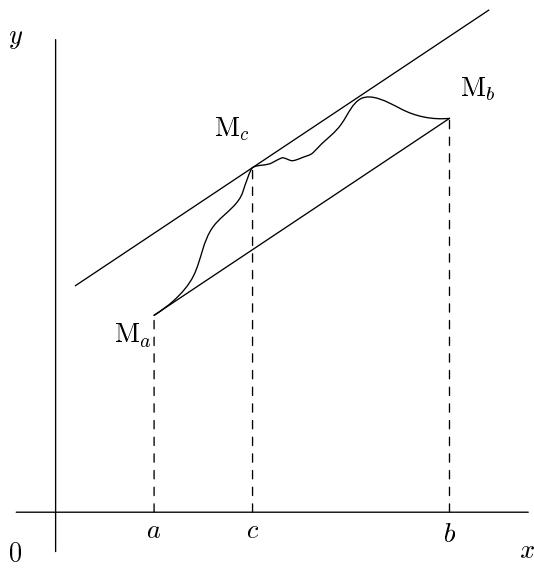
\includegraphics[keepaspectratio]{images/part001_3bcb0893.jpg}}\\
Fig. 4

the set \(\overline{g}(k)\) is closed and not empty (Gen.~Top., IV, p.~361, th. 3 and prop. 1). Let c be the greatest lower bound of \(\overline{g}(k)\) ; we have a \textless{} c \textless{} b, and at the point \(M_{c}\) the line D with equation \(y = f(c) + \frac{f(b) - f(a)}{b - a}(x - c)\) lies locally above G; but it cannot be locally on G at this point, since, for a \textless{} x \textless{} c, one has \(g(x) < k\) , which signifies that \(M_{x}\) is strictly below D. This has led us to a contradiction, which establishes the proposition.

COROLLARY 1. For a real finite function \(f\) defined on an open interval \(\mathbf{I} \subset \mathbf{R}\) and upper semi-continuous on \(\mathbf{I}\) to be convex on \(\mathbf{I}\) it is necessary and sufficient that for all \(x \in \mathbf{I}\) there should exist an \(\varepsilon > 0\) such that the relation \(|h| \leqslant \varepsilon\) entails

\[
f (x) \leqslant \frac {1}{2} (f (x + h) + f (x - h)).
\]

We have only to show that the condition is sufficient. Indeed, if at a point \(M_{a}\) of the graph G of f a line D is locally above G, then it is locally on G at this point; for, in the opposite case, for example, a point \(M_{a+h}\) would be strictly below D, while a point \(M_{a-h}\) would be below D; the mid-point of the segment \(M_{a-h}M_{a+h}\) would thus be strictly above D (fig.~5), and, in virtue of the hypothesis, \(M_{a}\) would a fortiori be strictly below D, which is absurd.

\pandocbounded{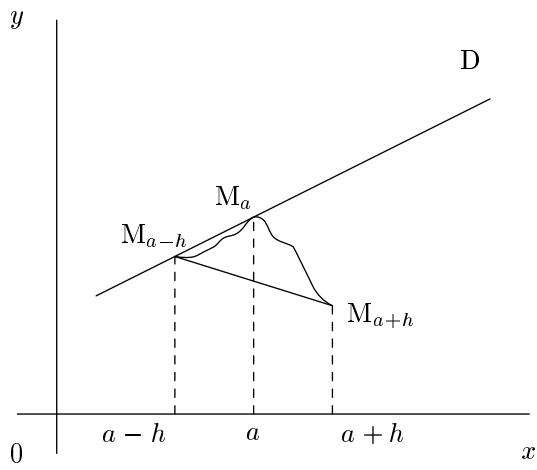
\includegraphics[keepaspectratio]{images/part001_b7dc5930.jpg}}\\
Fig. 5

COROLLARY 2. Let \(f\) be a finite real function defined on an open interval \(\mathrm{I} \subset \mathbf{R}\) . If for every point \(x \in \mathrm{I}\) there is an open interval \(\mathrm{J}_x \subset \mathrm{I}\) containing \(x\) and such that the restriction of \(f\) to \(\mathrm{J}_x\) is convex on \(\mathrm{J}_x\) , then \(f\) is convex on \(\mathrm{I}\) .

It is clear that \(f\) satisfies the criterion of prop. 9.

\setcounter{exercisegroup}{0}
\refstepcounter{exercisegroup}
\section*{Exercises on \S\arabic{exercisegroup}}
\phantomsection
\addcontentsline{toc}{section}{Exercises on \protect\S\arabic{exercisegroup}}

\begin{enumerate}
\def\labelenumi{\arabic{enumi})}
\tightlist
\item
  Let \(f\) be a vector function of a real variable, defined on an interval \(I \subset \mathbf{R}\) and differentiable at a point \(x_0\) interior to \(I\) . Show that the quotient
\end{enumerate}

\[
\frac {f (x _ {0} + h) - f (x _ {0} - k)}{h + k}
\]

tends to \(f'(x_0)\) as \(h\) and \(k\) tend to 0 through values \(> 0\) . Converse.

*Show that the function \(f\) equal to \(x^2 \sin 1/x\) for \(x \neq 0\) , and to 0 for \(x = 0\) , is everywhere differentiable, but that \((f(y) - f(z)) / (y - z)\) does not approach \(f'(0)\) as \(y\) and \(z\) tend to 0, while remaining distinct and \(>0_*\)

\begin{enumerate}
\def\labelenumi{\arabic{enumi})}
\setcounter{enumi}{1}
\tightlist
\item
  On the interval I = {[}0, 1{]} we define a sequence of continuous real functions \((f_{n})\) inductively as follows: We take \(f_{0}(x) = x\) ; for each integer \(n \geqslant 1\) the function \(f_{n}\) is affine linear on each of the \(3^{n}\) intervals \(\left[\frac{k}{3^{n}}, \frac{k+1}{3^{n}}\right]\) for \(0 \leqslant k \leqslant 3^{n}-1\) ; further, we take
\end{enumerate}

\[
f _ {n + 1} \left(\frac {k}{3 ^ {n}}\right) = f _ {n} \left(\frac {k}{3 ^ {n}}\right)
\]

\[
f _ {n + 1} \left(\frac {k}{3 ^ {n}} + \frac {1}{3 ^ {n + 1}}\right) = f _ {n} \left(\frac {k}{3 ^ {n}} + \frac {2}{3 ^ {n + 1}}\right), f _ {n + 1} \left(\frac {k}{3 ^ {n}} + \frac {2}{3 ^ {n + 1}}\right) = f _ {n} \left(\frac {k}{3 ^ {n}} + \frac {1}{3 ^ {n + 1}}\right).
\]

Show that the sequence \((f_{n})\) converges uniformly on I to a continuous function which has no derivative (finite or infinite) at any point of the interval {]}0, 1{[} (use exerc. 1).

\begin{enumerate}
\def\labelenumi{\arabic{enumi})}
\setcounter{enumi}{2}
\item
  Let \(\mathcal{C}(\mathrm{I})\) be the complete space of continuous finite real functions defined on the compact interval \(\mathrm{I} = [a,b]\) of \(\mathbf{R}\) , and endow \(\mathcal{C}(\mathrm{I})\) with the topology of uniform convergence (Gen.~Top., X, p.~277). Let A be the subset of \(\mathcal{C}(\mathrm{I})\) formed by the functions \(x\) such that for at least one point \(t\in [a,b[\) (depending on the function \(x\) ) the function \(x\) has a finite right derivative. Show that A is a meagre set in \(\mathcal{C}(\mathrm{I})\) (Gen.~Top., IX, p.~192), and hence its complement, that is, the set of continuous functions on I not having a finite right derivative at any point of \([a,b[\) is a Baire subspace of \(\mathcal{C}(\mathrm{I})\) (Gen.~Top., IX, p.~192). (Let \(\mathrm{A}_n\) be the set of functions \(x\in \mathcal{C}(\mathrm{I})\) such that for at least one value of \(t\) satisfying \(a\leqslant t\leqslant b - 1 / n\) (and depending on \(x\) ) one has \(|x(t') - x(t)|\leqslant n|t' - t|\) for all \(t'\) such that \(t\leqslant t'\leqslant t + 1 / n\) . Show that each \(\mathrm{A}_n\) is a closed nowhere dense set in \(\mathcal{C}(\mathrm{I})\) : remark that in \(\mathcal{C}(\mathrm{I})\) each ball contains a function having bounded right derivative on \([a,b[\) ; on the other hand, for every \(\varepsilon >0\) and every integer \(m > 0\) there exists on I a continuous function having at every point of \([a,b[\) a finite right derivative such that, for all \(t\in [a,b[\) one has \(|y(t)|\leqslant \varepsilon\) and \(|y_r'(t)|\geqslant m\) .)
\item
  Let E be a topological vector space over R and f a continuous vector function defined on an open interval \(I \subset R\) , and having a right derivative and a left derivative at every point of I.
\end{enumerate}

\begin{enumerate}
\def\labelenumi{\alph{enumi})}
\item
  Let U be a nonempty open set in E, and A the subset of I formed by the points x such that \(\mathbf{f}_{d}^{\prime}(x) \in \mathrm{U}\) . Given a number \(\alpha > 0\) let B be the subset of I formed by the points x such that there exists at least one \(y \in I\) satisfying the conditions \(x - \alpha \leqslant y < x\) and \((\mathbf{f}(x) - \mathbf{f}(y)) / (x - y) \in \mathrm{U}\) ; show that the set B is open and that \(A \cap CB\) is countable (remark that this last set is formed by the left-hand endpoints of intervals contiguous to CB). Deduce that the set of points \(x \in A\) such that \(\mathbf{f}_{g}^{\prime}(x) \notin \overline{\mathbf{U}}\) is countable.
\item
  Suppose that E is a normed space; the image \(\mathbf{f}(\mathrm{I})\) is then a metric space having a countable base, and the same is true for the closed vector subspace F of E generated by \(\mathbf{f}(\mathrm{I})\) , a subspace which contains \(\mathbf{f}_{d}^{\prime}(\mathrm{I})\) and \(\mathbf{f}_{g}^{\prime}(\mathrm{I})\) . Deduce from a) that the set of points \(x \in I\) such that \(\mathbf{f}_{d}^{\prime}(x) \neq \mathbf{f}_{g}^{\prime}(x)\) is countable. (If \((\mathrm{U}_{m})\) is a countable base for the topology of F note that for two distinct points a, b of F there exist two disjoint sets \(U_{p}, U_{q}\) such that \(a \in U_{p}\) and \(b \in U_{q}\) .)
\item
  Take for E the product \(R^{I}\) (the space of mappings from I into R, endowed with the topology of simple convergence), and for each \(x \in I\) denote by \(\mathbf{g}(x)\) the map \(t \mapsto |x - t|\) of I into R. Show that g is continuous and that, for every \(x \in I\) , one has \(\mathbf{g}_{r}'(x) \neq \mathbf{g}_{l}'(x)\) .
\end{enumerate}

\begin{enumerate}
\def\labelenumi{\arabic{enumi})}
\setcounter{enumi}{4}
\tightlist
\item
  Let \(\mathbf{f}\) be a continuous vector function defined on an open interval \(\mathrm{I} \subset \mathbf{R}\) with values in a normed space \(\mathrm{E}\) over \(\mathbf{R}\) , and admitting a right derivative at every point of \(\mathrm{I}\) .
\end{enumerate}

\begin{enumerate}
\def\labelenumi{\alph{enumi})}
\item
  Show that the set of points \(x \in \mathrm{I}\) such that \(\mathbf{f}_d'\) is bounded on a neighbourhood of \(x\) is an open set dense in \(\mathrm{I}\) (use th. 2 of Gen.~Top., IX, p.~194).
\item
  Show that the set of points of I where \(\mathbf{f}_d^{\prime}\) is continuous is the complement of a meagre subset of I (cf.~Gen.~Top., IX, p.~255, exerc. 21).
\end{enumerate}

\begin{enumerate}
\def\labelenumi{\arabic{enumi})}
\setcounter{enumi}{5}
\tightlist
\item
  Let \((r_n)\) be the sequence formed by the rational numbers in {[}0, 1{]}, arranged in a certain order. Show that the function \(f(x) = \sum_{n=0}^{\infty} 2^{-n}(x - r_n)^{1/3}\) is continuous and differentiable
\end{enumerate}

at every point of \(\mathbf{R}\) , and has an infinite derivative at every point \(r_n\) . (To see that \(f\) is differentiable at a point \(x\) distinct from the \(r_n\) , distinguish two cases, according to whether the series with general term \(2^{-n}(x - r_n)^{-2/3}\) has sum \(+\infty\) or converges; in the second case, note for all \(x \neq 0\) and all \(y \neq x\) , one has

\[
0 \leqslant (y ^ {1 / 3} - x ^ {1 / 3}) / (y - x) \leqslant 4 / 3 x ^ {2 / 3}).
\]

\begin{enumerate}
\def\labelenumi{\arabic{enumi})}
\setcounter{enumi}{6}
\item
  Let \(f\) be a real function defined on an interval \(\mathrm{I} \subset \mathbf{R}\) , admitting a right derivative \(f_d'(x_0) = 0\) at a point of \(\mathrm{I}\) , and let \(\mathbf{g}\) be a vector function defined on a neighbourhood of \(y_0 = f(x_0)\) , having a right derivative and a left derivative (not necessarily equal) at this point. Show that \(\mathbf{g} \circ f\) has a right derivative equal to 0 at the point \(x_0\) .
\item
  Let \(f\) be a mapping from \(\mathbf{R}\) to itself such that the set \(C\) of points of \(\mathbf{R}\) where \(f\) is continuous is dense in \(\mathbf{R}\) , and such that the complement \(A\) of \(C\) is also dense. Show that the set \(D\) of points of \(C\) where \(f\) is right differentiable is meagre. (For each integer \(n\) , let \(E_n\) be the set of points \(a \in \mathbf{R}\) such that there exist two points \(x, y\) such that \(0 < x - a < 1/n\) , \(0 < y - a < 1/n\) and
\end{enumerate}

\[
\frac {f (x) - f (a)}{x - a} - \frac {f (y) - f (a)}{y - a} > 1.
\]

Show that the interior of \(E_{n}\) is dense in R. For this, note that for every open nonempty interval I in R there is a point \(b \in I \cap A\) ; show that for a \textless{} b and b - a sufficiently small one has \(a \in E_{n}\) .

\begin{enumerate}
\def\labelenumi{\arabic{enumi})}
\setcounter{enumi}{8}
\tightlist
\item
  Let \(\mathcal{B}(\mathbf{N})\) be the space of bounded sequences \(\mathbf{x} = (x_n)_{n\in \mathbb{N}}\) of real numbers, endowed with the norm \(\| \mathbf{x}\| = \sup |x_n|\) ; give an example of a continuous map \(t\mapsto \mathbf{f}(t) = (f_n(t))_{n\in \mathbb{N}}\) of \(\mathbf{R}\) into \(\mathcal{B}(\mathbf{N})\) such that each of the functions \(f_{n}\) is differentiable for \(t = 0\) , but \(\mathbf{f}\) is not differentiable at this point.
\end{enumerate}

\setcounter{exercisegroup}{1}
\refstepcounter{exercisegroup}
\section*{Exercises on \S\arabic{exercisegroup}}
\phantomsection
\addcontentsline{toc}{section}{Exercises on \protect\S\arabic{exercisegroup}}

\begin{enumerate}
\def\labelenumi{\arabic{enumi})}
\item
  Let \(f\) be a real function defined and left continuous on an open interval \(I = ]a, b[\) in \(R\) ; suppose that at all the points of the complement \(B\) with respect to \(I\) of a countable subset of \(I\) the function \(f\) is increasing to the right, that is, at every point \(x \in B\) there exists a \(y\) such that \(x < y \leqslant b\) and such that for all \(z\) such that \(x \leqslant z < y\) one has \(f(x) \leqslant f(z)\) . Show that \(f\) is increasing on \(I\) (argue as in prop. 2).
\item
  In the field \(Q_{p}\) of p-adic numbers (Gen.~Top., III, p.~322, exerc. 23) every p-adic integer \(x \in Z_{p}\) has one and only one expansion in the form \(x = a_{0} + a_{1}p + \cdots + a_{n}p^{n} + \cdots\) , where the \(a_{j}\) are rational integers such that \(0 \leqslant a_{j} \leqslant p - 1\) for each j. For each \(z \in Z_{p}\) put
\end{enumerate}

\[
f (x) = a _ {0} + a _ {1} p ^ {2} + \dots + a _ {n} p ^ {2 n} + \dots ;
\]

show that, on \(Z_{p}\) , f is a continuous function which is not constant on a neighbourhood of any point yet has a zero derivative at every point.

\begin{enumerate}
\def\labelenumi{\arabic{enumi})}
\setcounter{enumi}{2}
\tightlist
\item
  \begin{enumerate}
  \def\labelenumii{\alph{enumii})}
  \tightlist
  \item
    Let K be the triadic Cantor set (Gen.~Top., IV, p.~338), let \(I_{n,p}\) be the \(2^{n}\) contiguous intervals of K with length \(1/3^{n+1}\) ( \(1 \leqslant p \leqslant 2^{n}\) ), and \(K_{n,p}\) the \(2^{n+1}\) closed intervals of length \(1/3^{n+1}\) whose union is the complement of the union of the \(I_{m,p}\) for \(m \leqslant n\) . Let \(\alpha\) be a number such that \(1 < \alpha < 3/2\) ; for each n we denote by \(f_{n}\) the continuous increasing function on {[}0, 1{]} which is equal to 0 for x = 0, constant on each of the intervals \(I_{m,p}\) for \(m \leqslant n\) , is affine linear on each of the intervals \(K_{n,p}\) ( \(1 \leqslant p \leqslant 2^{n+1}\) ) and such that \(f_{d}'(x) = \alpha^{n+1}\) on each of the interiors of these last intervals. Show that the series with general term \(f_{n}\) is uniformly convergent on {[}0, 1{]}, that its sum is a function f which admits a right derivative (finite or not) everywhere in {[}0, 1{[}, and that one has \(f_{r}'(x) = +\infty\) at every point of K distinct from the left-hand endpoints of the contiguous intervals \(I_{n,p}\) .
  \end{enumerate}
\end{enumerate}

\begin{enumerate}
\def\labelenumi{\alph{enumi})}
\setcounter{enumi}{1}
\tightlist
\item
  Let g be a continuous increasing map of \([0, 1]\) onto itself, constant on each of the intervals \(I_{n,p}\) (Gen.~Top., IV, p.~403, exerc. 9). If \(h = f + g\) , show that h admits a right derivative equal to \(f_{d}^{\prime}(x)\) at every point x of \([0, 1]\) .
\end{enumerate}

\begin{enumerate}
\def\labelenumi{\arabic{enumi})}
\setcounter{enumi}{3}
\tightlist
\item
  Let \(f\) be a finite real function, continuous on a compact interval \([a, b]\) in \(\mathbf{R}\) , and having a right derivative at every point of the open interval \(]a, b[\) . Let \(m\) and \(M\) be the greatest lower bound and least upper bound (finite or not) of \(f_d'\) over \(]a, b[\) .
\end{enumerate}

\begin{enumerate}
\def\labelenumi{\alph{enumi})}
\item
  Show that when x and y run through {]}a, b{[} keeping \(x \neq y\) , the set of values of \((f(x) - f(y))/(x - y)\) contains {]}m, M{[} and is contained in {[}m, M{]}. (Reduce to proving that if \(f_{d}^{\prime}\) takes two values of opposite sign at the two points c, d of {]}a, b{[} (with c \textless{} d), then there exist two distinct points of the interval {]}c, d{[} where f takes the same value).
\item
  If, further, f has a left derivative at every point of \(]a\) , b{[} then the infima (resp. suprema) of \(f_{d}^{\prime}\) and \(f_{g}^{\prime}\) over \(]a\) , b{[} are equal.
\item
  Deduce that if \(f\) is differentiable on \(]a, b[\) then the image under \(f'\) of every interval contained in \(]a, b[\) is itself an interval, and consequently connected (use \(a\) ).
\end{enumerate}

\begin{enumerate}
\def\labelenumi{\arabic{enumi})}
\setcounter{enumi}{4}
\item
  Let \(\mathbf{f}\) be the vector mapping of \(I = [0, 1]\) into \(\mathbf{R}^3\) defined as follows: for \(0 \leqslant t \leqslant \frac{1}{4}\) , \(\mathbf{f}(t) = (-4t, 0, 0)\) ; for \(\frac{1}{4} \leqslant t \leqslant \frac{1}{2}\) let \(\mathbf{f}(t) = (-1, 4t - 1, 0)\) ; for \(\frac{1}{2} \leqslant t \leqslant \frac{3}{4}\) let \(\mathbf{f}(t) = (-1, 1, 4t - 2)\) ; finally, for \(\frac{3}{4} \leqslant t \leqslant 1\) take \(\mathbf{f}(t) = (4t - 4, 1, 1)\) . Show that the convex set generated by the set \(\mathbf{f}_d'(\mathrm{I})\) is not identical to the closure of the set of values of \(\frac{\mathbf{f}(y) - \mathbf{f}(x)}{y - x}\) as \((x, y)\) runs through the set of pairs of distinct points of \(I\) (cf.~exerc. \(4a\) )).
\item
  On the interval \(\mathbf{I} = [-1, + 1]\) consider the vector function \(\mathbf{f}\) , with values in \(\mathbf{R}^2\) , defined as follows: \(\mathbf{f}(t) = (0,0)\) for \(-1\leqslant t\leqslant 0\) ;
\end{enumerate}

\[
\mathbf {f} (t) = \left(t ^ {2} \sin \frac {1}{t}, t ^ {2} \cos \frac {1}{t}\right)
\]

for \(0 \leqslant t \leqslant 1\) . Show that \(\mathbf{f}\) is differentiable on \([-1, +1[\) but that the image of this interval under \(\mathbf{f}'\) is not a connected set in \(\mathbf{R}^2\) ( \(cf.\) exerc. \(4c\) )).

\begin{enumerate}
\def\labelenumi{\arabic{enumi})}
\setcounter{enumi}{6}
\item
  Let f be a continuous vector function defined on an open interval \(I \subset R\) , with values in a normed space E over R, and admitting a right derivative at every point of I. Show that the set of points of I where f admits a derivative is the complement of a meagre subset of I (use exerc. 5 b) of I, p.~36, and prop. 6 of I, p.~18).
\item
  Consider, on the interval {[}0, 1{]}, a family \((\mathrm{I}_{n,p})\) of pairwise disjoint open intervals, defined inductively as follows: the integer \(n\) takes all values \(\geqslant 0\) ; for each value of \(n\) the integer \(p\) takes the values \(1,2,\ldots ,2^n\) ; one has \(\mathrm{I}_{0,1} = ]\frac{1}{3},\frac{2}{3}[\) ; if \(\mathrm{J}_n\) is the union of the intervals \(\mathrm{I}_{m,p}\) corresponding to the numbers \(m\leqslant n\) , the complement of \(\mathrm{J}_n\) is the union of \(2^{n + 1}\) pairwise disjoint closed intervals \(\mathrm{K}_{n,p}\) ( \(1\leqslant p\leqslant 2^{n + 1}\) ). If \(\mathrm{K}_{n,p}\) is an interval \([a,b]\) one then takes for \(\mathrm{I}_{n + 1,p}\) the open interval with endpoints \(b - \frac{b - a}{3}\left(1 + \frac{1}{2^n}\right)\) and \(b - \frac{b - a}{3.2^n}\) . Let E be the perfect set which is the complement with respect to {[}0, 1{]} of the union of the \(\mathrm{I}_{n,p}\) . Define on {[}0, 1{]} a continuous real function \(f\) which admits a right derivative at every point of {[}0, 1{]}, but fails to have a left derivative at the uncountable subset of E of points distinct from the endpoints of intervals contiguous to E (cf.~exerc. 7). (Take \(f(x) = 0\) on E, define \(f\) suitably on each of the intervals \(\mathrm{I}_{n,p}\) in such a way that for every \(x\in \mathrm{E}\) there are points \(y < x\) not belonging to E, arbitrarily close to \(x\) , and such that \(\frac{f(y) - f(x)}{y - x} = -1\) .)
\item
  Let \(f\) and \(g\) be two finite real functions, continuous on \([a, b]\) , both having a finite derivative on \(]a, b[\) ; show that there exists a \(c\) such that \(a < c < b\) and that
\end{enumerate}

\[
\left| \begin{array}{c c} f (b) - f (a) & g (b) - g (a) \\ f ^ {\prime} (c) & g ^ {\prime} (c) \end{array} \right| = 0.
\]

¶ 10) Let \(f\) and \(g\) be two finite real functions, strictly positive, continuous and differentiable on an open interval I. Show that if \(f'\) and \(g'\) are strictly positive and \(f'/g'\) is strictly increasing on I, then either \(f/g\) is strictly increasing on I, or else there exists a number \(c \in I\) such that \(f / g\) is strictly decreasing for \(x \leqslant c\) and strictly increasing for \(x \geqslant c\) (note that if one has \(f'(x) / g'(x) < f(x) / g(x)\) then also

\[
f ^ {\prime} (y) / g ^ {\prime} (y) <   f (y) / g (y)
\]

for all y \textless{} x).

\begin{enumerate}
\def\labelenumi{\arabic{enumi})}
\setcounter{enumi}{10}
\tightlist
\item
  Let \(f\) be a complex function, continuous on an open interval \(I\) , vanishing nowhere, and admitting a right derivative at every point of \(I\) . For \(|f|\) to be increasing on \(I\) it is necessary and sufficient that \(\mathcal{R}(f_d' / f) \geqslant 0\) on \(I\) .
\end{enumerate}

¶ 12) Let \(f\) be a differentiable real function on an open interval I, \(g\) its derivative on I, and \([a, b]\) a compact interval contained in I; suppose that \(g\) is differentiable on the open interval \([a, b]\) but not necessarily right (resp. left) continuous at the point \(a\) (resp. \(b\) ); show that there exists \(c\) such that \(a < c < b\) and that

\[
g (b) - g (a) = (b - a) g ^ {\prime} (c)
\]

(use exerc. 4 c) of I, p.~36).

\begin{enumerate}
\def\labelenumi{\arabic{enumi})}
\setcounter{enumi}{12}
\tightlist
\item
  One terms the symmetric derivative of a vector function \(\mathbf{f}\) at a point \(x_0\) interior to the interval where \(\mathbf{f}\) is defined, the limit (when it exists) of \(\frac{\mathbf{f}(x_0 + h) - \mathbf{f}(x_0 - h)}{2h}\) as \(h\) tends to 0 remaining \(>0\) .
\end{enumerate}

\begin{enumerate}
\def\labelenumi{\alph{enumi})}
\item
  Generalize to the symmetric derivative the rules of calculus established in § 1 for the derivative.
\item
  Show that theorems 1 and 2 of § 2 remain valid when one replaces the words ``right derivative'' by ``symmetric derivative''.
\end{enumerate}

\begin{enumerate}
\def\labelenumi{\arabic{enumi})}
\setcounter{enumi}{13}
\tightlist
\item
  Let \(\mathbf{f}\) be a vector function defined and continuous on a compact interval \(\mathrm{I} = [a, b]\) in \(\mathbf{R}\) , with values in a normed space over \(\mathbf{R}\) . Suppose that \(\mathbf{f}\) admits a right derivative at all points of the complement with respect to \([a, b[\) of a countable subset A of this interval. Show that there exists a point \(x \in ]a\) , \(b[\cap ∁A\) such that
\end{enumerate}

\[
\left\| \mathbf {f} (b) - \mathbf {f} (a) \right\| \leqslant \left\| \mathbf {f} _ {d} ^ {\prime} (x) \right\| (b - a).
\]

(Argue by contradiction, decomposing \([a, b[\) into three intervals \([a, t[, [t, t + h[\) and \([t + h, b[\) with \(t \notin A\) ; if \(k = \| \mathbf{f}(b) - \mathbf{f}(a)\| / (b - a)\) , note that for \(h\) sufficiently small one has \(\| \mathbf{f}(t + h) - \mathbf{f}(t)\| < k.h\) , and use th. 2 of I, p.~15 for the other intervals.)

\setcounter{exercisegroup}{2}
\refstepcounter{exercisegroup}
\section*{Exercises on \S\arabic{exercisegroup}}
\phantomsection
\addcontentsline{toc}{section}{Exercises on \protect\S\arabic{exercisegroup}}

\begin{enumerate}
\def\labelenumi{\arabic{enumi})}
\tightlist
\item
  With the same hypotheses as in prop. 2 of I, p.~20 prove the formula
\end{enumerate}

\[
[ \mathbf {f} ^ {(n)}. \mathbf {g} ] = \sum_ {p = 0} ^ {n} (- 1) ^ {p} \binom {n} {p} D ^ {n - p} [ \mathbf {f}. \mathbf {g} ^ {(p)} ].
\]

\begin{enumerate}
\def\labelenumi{\arabic{enumi})}
\setcounter{enumi}{1}
\tightlist
\item
  With the notation of prop. 2 of I, p.~28 suppose that the relation \([\mathbf{a}.\mathbf{y}] = 0\) for all \(\mathbf{y} \in \mathrm{F}\) implies that \(\mathbf{a} = 0\) in E. Under these conditions, if \(\mathbf{g}_i\) ( \(0 \leqslant i \leqslant n\) ) are \(n + 1\) vector functions with values in E, defined on an interval I of R and such that for every vector function f with values in F and n times differentiable on I, one has identically
\end{enumerate}

\[
[ \mathbf {g} _ {0}. \mathbf {f} ] + [ \mathbf {g} _ {1}. \mathbf {f} ^ {\prime} ] + \dots + [ \mathbf {g} _ {n}. \mathbf {f} ^ {(n)} ] = 0
\]

then the functions \(g_{i}\) are identically zero.

\begin{enumerate}
\def\labelenumi{\arabic{enumi})}
\setcounter{enumi}{2}
\tightlist
\item
  With the notation of exerc. 2 and the same hypothesis on \([x.y]\) suppose that each of the functions \(g_{k}\) is n times differentiable on I; for each function f which is n times differentiable on I, with values in F, put
\end{enumerate}

\[
[ \mathbf {g} _ {0}. \mathbf {f} ] - [ \mathbf {g} _ {1}. \mathbf {f} ] ^ {\prime} + [ \mathbf {g} _ {2}. \mathbf {f} ] ^ {\prime \prime} + \dots + (- 1) ^ {n} [ \mathbf {g} _ {n}. \mathbf {f} ] ^ {(n)} = [ \mathbf {h} _ {0}. \mathbf {f} ] + [ \mathbf {h} _ {1}. \mathbf {f} ^ {\prime} ] + \dots + [ \mathbf {h} _ {n}. \mathbf {f} ^ {(n)} ],
\]

which defines the functions \(\mathbf{h}_i\) ( \(0 \leqslant i \leqslant n\) ) without ambiguity (exerc. 2); show that one has

\[
[ \mathbf {h} _ {0}. \mathbf {f} ] - [ \mathbf {h}. \mathbf {f} ] ^ {\prime} + [ \mathbf {h} _ {2}. \mathbf {f} ] ^ {\prime \prime} + \dots + (- 1) ^ {n} [ \mathbf {h} _ {n}. \mathbf {f} ] ^ {(n)} = [ \mathbf {g} _ {0}. \mathbf {f} ] + [ \mathbf {g} _ {1}. \mathbf {f} ^ {\prime} ] + \dots + [ \mathbf {g} _ {n}. \mathbf {f} ^ {(n)} ]
\]

identically.

\begin{enumerate}
\def\labelenumi{\arabic{enumi})}
\setcounter{enumi}{3}
\tightlist
\item
  Let \(\mathbf{f}\) be a vector function which is \(n\) times differentiable on an interval \(\mathrm{I} \subset \mathbf{R}\) . Show that for \(1 / x \in \mathrm{I}\) one has identically
\end{enumerate}

\[
\frac {1}{x ^ {n + 1}} \mathbf {f} ^ {(n)} \left(\frac {1}{x}\right) = (- 1) ^ {n} \mathrm{D} ^ {n} \left(x ^ {n - 1} \mathbf {f} \left(\frac {1}{x}\right)\right)
\]

(argue inductively on \(n\) ).

\begin{enumerate}
\def\labelenumi{\arabic{enumi})}
\setcounter{enumi}{4}
\tightlist
\item
  Let \(u\) and \(v\) be two real functions which are \(n\) times differentiable on an interval \(I \subset \mathbf{R}\) . If one puts \(D^n(u / v) = (-1)^n w_n / v^{n+1}\) at every point where \(v(x) \neq 0\) , show that
\end{enumerate}

\[
w _ {n} = \left| \begin{array}{c c c c c c} u & v & 0 & 0 & \dots & 0 \\ u ^ {\prime} & v ^ {\prime} & v & 0 & \dots & 0 \\ u ^ {\prime \prime} & v ^ {\prime \prime} & 2 v ^ {\prime} & v & \dots & 0 \\ \dots & \dots & \dots & \dots & \dots & \dots \\ u ^ {(n - 1)} & v ^ {(n - 1)} & \binom {n - 1} {1} v ^ {(n - 2)} & \binom {n - 1} {2} v ^ {(n - 3)} & \dots & v \\ u ^ {(n)} & v ^ {(n)} & \binom {n} {1} v ^ {(n - 1)} & \binom {n} {2} v ^ {(n - 2)} & \dots & \binom {n} {n - 1} v ^ {\prime} \end{array} \right|
\]

(put \(w = u / v\) and differentiate \(n\) times the relation \(u = wv\) ).

\begin{enumerate}
\def\labelenumi{\arabic{enumi})}
\setcounter{enumi}{5}
\tightlist
\item
  Let \(\mathbf{f}\) be a vector function defined on an open interval \(\mathrm{I} \subset \mathbf{R}\) , taking values in a normed space \(\mathrm{E}\) .
\end{enumerate}

Put \(\Delta \mathbf{f}(x; h_1) = \mathbf{f}(x + h_1) - \mathbf{f}(x)\) , and then, inductively, define

\[
\Delta^ {p} \mathbf {f} (x; h _ {1}, h _ {2}, \dots , h _ {p - 1}, h _ {p}) = \Delta^ {p - 1} \mathbf {f} (x + h _ {p}; h _ {1}, \dots , h _ {p - 1}) - \Delta^ {p - 1} \mathbf {f} (x; h _ {1}, \dots , h _ {p - 1});
\]

these functions are defined for each \(x \in I\) when the \(h_{i}\) are small enough.

\begin{enumerate}
\def\labelenumi{\alph{enumi})}
\tightlist
\item
  If the function \(\mathbf{f}\) is \(n\) times differentiable at the point \(x\) (and so \(n - 1\) times differentiable on a neighbourhood of \(x\) ), one has
\end{enumerate}

\[
\lim_{\substack{(h_{1},\ldots ,h_{n})\to (0,\ldots ,0)\\ h_{1}h_{2}\ldots h_{n}\neq 0}}\frac{\varDelta^{n}\mathbf{f}(x;h_{1},\ldots,h_{n})}{h_{1}h_{2}\ldots h_{n}} = \mathbf{f}^{(n)}(x)
\]

(argue by induction on n, using the mean value theorem).

\begin{enumerate}
\def\labelenumi{\alph{enumi})}
\setcounter{enumi}{1}
\tightlist
\item
  If \(\mathbf{f}\) is \(n\) times differentiable on the interval I, one has
\end{enumerate}

\[
\begin{array}{l} \left\| \Delta^ {n} \mathbf {f} (x; h _ {1}, \ldots , h _ {n}) - \mathbf {f} ^ {(n)} (x _ {0}) h _ {1} h _ {2} \ldots h _ {n} \right\| \\ \leqslant | h _ {1} h _ {2} \ldots h _ {n} | \sup \left\| \mathbf {f} ^ {(n)} (x + t _ {1} h _ {1} + \dots + t _ {n} h _ {n}) - \mathbf {f} ^ {(n)} (x _ {0}) \right\| \end{array}
\]

the supremum being taken over the set of \((t_i)\) such that \(0 \leqslant t_i \leqslant 1\) for \(1 \leqslant i \leqslant n\) (same method).

\begin{enumerate}
\def\labelenumi{\alph{enumi})}
\setcounter{enumi}{2}
\tightlist
\item
  If \(f\) is a real function which is \(n\) times differentiable on I, one has
\end{enumerate}

\[
\Delta^ {n} f (x; h _ {1}, h _ {2}, \dots , h _ {n}) = h _ {1} h _ {2} \dots h _ {n} f ^ {(n)} (x + \theta_ {1} h _ {1} + \dots + \theta_ {n} h _ {n})
\]

the numbers \(\theta_{i}\) belonging to {[}0, 1{]} (same method, using I, p.~22, corollary).

\begin{enumerate}
\def\labelenumi{\arabic{enumi})}
\setcounter{enumi}{6}
\tightlist
\item
  Let \(f\) be a finite real function \(n\) times differentiable at the point \(x_0\) , and \(\mathbf{g}\) a vector function which is \(n\) times differentiable at the point \(y_0 = f(x_0)\) . Let
\end{enumerate}

\[
\begin{array}{l} f (x _ {0} + h) = a _ {0} + a _ {1} h + \dots + a _ {n} h ^ {n} + r _ {n} (h) \\ \mathbf {g} (y _ {0} + k) = \mathbf {b} _ {0} + \mathbf {b} _ {1} k + \dots + \mathbf {b} _ {n} k ^ {n} + \mathbf {s} _ {n} (k) \end{array}
\]

be the Taylor expansions of order n of f and g at the points \(x_{0}\) and \(y_{0}\) respectively. Show that the sum of the \(n+1\) terms of the Taylor expansion of order n of the composite function \(g \circ f\) at the point \(x_{0}\) is equal to the sum of the terms of degree \(\leqslant n\) in the polynomial

\[
\mathbf {b} _ {0} + \mathbf {b} _ {1} (a _ {1} h + \dots + a _ {n} h ^ {n}) + \mathbf {b} _ {2} (a _ {1} h + \dots + a _ {n} h ^ {n}) ^ {2} + \dots + \mathbf {b} _ {n} (a _ {1} h + \dots + a _ {n} h ^ {n}) ^ {n}.
\]

Deduce the two following formulae:

\begin{enumerate}
\def\labelenumi{\alph{enumi})}
\tightlist
\item
\end{enumerate}

\[
\mathrm{D} ^ {n} (\mathbf {g} (f (x))) = \sum \frac {n !}{m _ {1} ! m _ {2} ! \dots m _ {q} !} \mathbf {g} ^ {(p)} (f (x)) \left(\frac {f ^ {\prime} (x)}{1 !}\right) ^ {m _ {1}} \dots \left(\frac {f ^ {(q)} (x)}{q !}\right) ^ {m _ {q}}
\]

the sum being taken over all systems of positive integers \((m_{i})_{1\leqslant i\leqslant q}\) such that

\[
m _ {1} + 2 m _ {2} + \dots + q m _ {q} = n
\]

where p denotes the sum \(m_{1} + m_{2} + \cdots + m_{q}\) .

\begin{enumerate}
\def\labelenumi{\alph{enumi})}
\setcounter{enumi}{1}
\tightlist
\item
\end{enumerate}

\[
\mathrm{D} ^ {n} (\mathbf {g} (f (x))) = \sum_ {p = 1} ^ {n} \frac {1}{p !}   \mathbf {g} ^ {(p)} (f (x)) \left(\sum_ {q = 1} ^ {p} \binom {p} {q} (- f (x)) ^ {p - q}   \mathrm{D} ^ {n} ((f (x)) ^ {q}\right).
\]

\begin{enumerate}
\def\labelenumi{\arabic{enumi})}
\setcounter{enumi}{7}
\tightlist
\item
  Let \(f\) be a real function defined and \(n\) times differentiable on an interval \(\mathrm{I}\) , let \(x_{1}, x_{2}, \ldots, x_{p}\) be distinct points of \(\mathrm{I}\) , and \(n_{i}\) ( \(1 \leqslant i \leqslant p\) ) be \(p\) integers \(> 0\) such that
\end{enumerate}

\[
n _ {1} + n _ {2} + \dots + n _ {p} = n.
\]

Suppose that at the point \(x_{i}\) the function f vanishes together with its first \(n_{i}-1\) derivatives for \(1 \leqslant i \leqslant p\) : show that there is a point \(\xi\) interior to the smallest interval that contains the \(x_{i}\) and such that \(f^{(n-1)}(\xi) = 0\) .

\begin{enumerate}
\def\labelenumi{\arabic{enumi})}
\setcounter{enumi}{8}
\tightlist
\item
  With the same notation as in exerc. 8 suppose that \(f\) is \(n\) times differentiable on I but otherwise arbitrary. Let \(g\) be the polynomial of degree \(n - 1\) (with real coefficients) such that at the point \(x_{i}\) ( \(1 \leqslant i \leqslant p\) ) both \(g\) and its first \(n_{i} - 1\) derivatives are respectively equal to \(f\) and its first \(n_{i} - 1\) derivatives. Show that we have
\end{enumerate}

\[
f (x) = g (x) + \frac {(x - x _ {1}) ^ {n _ {1}} (x - x _ {2}) ^ {n _ {2}} \dots (x - x _ {p}) ^ {n _ {p}}}{n !} f ^ {(n)} (\xi)
\]

where \(\xi\) is interior to the smallest interval containing the points \(x_{i}\) ( \(1 \leqslant i \leqslant p\) ) and \(x\) . (Apply exerc. 8 to the function of \(t\)

\[
f (t) - g (t) - a \frac {(t - x _ {1}) ^ {n _ {1}} (t - x _ {2}) ^ {n _ {2}} \dots (t - x _ {p}) ^ {n _ {p}}}{n !}
\]

where \(a\) is a suitably chosen constant.)

\begin{enumerate}
\def\labelenumi{\arabic{enumi})}
\setcounter{enumi}{9}
\tightlist
\item
  Let \(g\) be an odd real function defined on a neighbourhood of 0, and 5 times differentiable on this neighbourhood. Show that
\end{enumerate}

\[
g (x) = \frac {x}{3} \left(g ^ {\prime} (x) + 2 g ^ {\prime} (0)\right) - \frac {x ^ {5}}{1 8 0} g ^ {(5)} (\xi) \quad (\xi = \theta x, \quad 0 <   \theta <   1)
\]

(same method as in exerc. 9).

Deduce that if \(f\) is a real function defined on \([a, b]\) and 5 times differentiable on this interval, then

\[
f (b) - f (a) = \frac {b - a}{6} \left[ f ^ {\prime} (a) + f ^ {\prime} (b) + 4 f ^ {\prime} \left(\frac {a + b}{2}\right) \right] - \frac {(b - a) ^ {5}}{2 8 8 0} f ^ {(5)} (\xi)
\]

with \(a < \xi < b\) (``Simpson's formula'').

\begin{enumerate}
\def\labelenumi{\arabic{enumi})}
\setcounter{enumi}{10}
\tightlist
\item
  Let \(f_{1}, f_{2}, \ldots, f_{n}\) and \(g_{1}, g_{2}, \ldots, g_{n}\) be \(2n\) real functions which are \(n - 1\) times differentiable on an interval I. Let \((x_{i})_{1 \leqslant i \leqslant n}\) be a strictly increasing sequence of points in I. Show that the ratio of the two determinants
\end{enumerate}

\[
\left| \begin{array}{c c c c} f _ {1} (x _ {1}) & f _ {1} (x _ {2}) & \dots & f _ {1} (x _ {n}) \\ f _ {2} (x _ {1}) & f _ {2} (x _ {2}) & \dots & f _ {2} (x _ {n}) \\ \dots & \dots & \dots & \dots \\ f _ {n} (x _ {1}) & f _ {n} (x _ {2}) & \dots & f _ {n} (x _ {n}) \end{array} \right| \vdots \left| \begin{array}{c c c c} g _ {1} (x _ {1}) & g _ {1} (x _ {2}) & \dots & g _ {1} (x _ {n}) \\ g _ {2} (x _ {1}) & g _ {2} (x _ {2}) & \dots & g _ {2} (x _ {n}) \\ \dots & \dots & \dots & \dots \\ g _ {n} (x _ {1}) & g _ {n} (x _ {2}) & \dots & g _ {n} (x _ {n}) \end{array} \right|
\]

is equal to the ratio of the two determinants

\[
\left| \begin{array}{c c c c} f _ {1} (\xi_ {1}) & f _ {1} ^ {\prime} (\xi_ {2}) & \dots & f _ {1} ^ {(n - 1)} (\xi_ {n}) \\ f _ {2} (\xi_ {1}) & f _ {2} ^ {\prime} (\xi_ {2}) & \dots & f _ {2} ^ {(n - 1)} (\xi_ {n}) \\ \dots & \dots & \dots & \dots \\ f _ {n} (\xi_ {1}) & f _ {n} ^ {\prime} (\xi_ {2}) & \dots & f _ {n} ^ {(n - 1)} (\xi_ {n}) \end{array} \right|: \left| \begin{array}{c c c c} g _ {1} (\xi_ {1}) & g _ {1} ^ {\prime} (\xi_ {2}) & \dots & g _ {1} ^ {(n - 1)} (\xi_ {n}) \\ g _ {2} (\xi_ {1}) & g _ {2} ^ {\prime} (\xi_ {2}) & \dots & g _ {2} ^ {(n - 1)} (\xi_ {n}) \\ \dots & \dots & \dots & \dots \\ g _ {n} (\xi_ {1}) & g _ {n} ^ {\prime} (\xi_ {2}) & \dots & g _ {n} ^ {(n - 1)} (\xi_ {n}) \end{array} \right|
\]

where

\[
\xi_ {1} = x _ {1}, \quad \xi_ {1} <   \xi_ {2} <   x _ {2}, \quad \xi_ {2} <   \xi_ {3} <   x _ {3}, \quad \dots , \quad \xi_ {n - 1} <   \xi_ {n} <   x _ {n}
\]

(apply exerc. 9 of I, p.~38).

Particular case where \(g_{1}(x)=1\) , \(g_{2}(x)=x,\ldots,g_{n}(x)=x^{n-1}\) .

¶ 12) \(a)\) Let \(\mathbf{f}\) be a vector function defined and continuous on the finite interval \(\mathrm{I} = [-a, + a]\) , taking its values in a normed space \(\mathrm{E}\) over \(\mathbf{R}\) and twice differentiable on \(\mathrm{I}\) . If one puts \(\mathrm{M}_0 = \sup_{x\in \mathrm{I}}\| \mathbf{f}(x)\|\) , \(\mathrm{M}_2 = \sup_{x\in \mathrm{I}}\| \mathbf{f}''(x)\|\) , show that for all \(x\in \mathrm{I}\) one has

\[
\left\| \mathbf {f} ^ {\prime} (x) \right\| \leqslant \frac {\mathrm{M} _ {0}}{a} + \frac {x ^ {2} + a ^ {2}}{2 a} \mathrm{M} _ {2}
\]

(express each of the differences \(\mathbf{f}(a) - \mathbf{f}(x)\) , \(\mathbf{f}(-a) - \mathbf{f}(x)\) ).

\begin{enumerate}
\def\labelenumi{\alph{enumi})}
\setcounter{enumi}{1}
\tightlist
\item
  Deduce from a) that if f is a twice differentiable function on an interval I (bounded or not), and if \(\mathbf{M}_{0} = \sup_{x \in I} \| \mathbf{f}(x) \|\) and \(\mathbf{M}_{2} = \sup_{x \in I} \| \mathbf{f}''(x) \|\) are finite, then so is \(\mathbf{M}_{1} = \sup_{x \in I} \| \mathbf{f}'(x) \|\) , and one has:
\end{enumerate}

\[
\mathrm{M} _ {1} \leqslant 2 \sqrt {\mathrm{M} _ {0} \mathrm{M} _ {2}} \quad \text { if   I   has   length } \geqslant 2 \sqrt {\frac {M _ {0}}{\mathrm{M} _ {2}}}
\]

\[
\mathrm{M} _ {1} \leqslant \sqrt {2} \sqrt {\mathrm{M} _ {0} \mathrm{M} _ {2}} \quad \text { if } \mathrm{I} = \mathbf {R}.
\]

Show that in these two inequalities the numbers 2 and \(\sqrt{2}\) respectively cannot be replaced by smaller numbers (consider first the case where one supposes merely that f admits a second right derivative, and show that in this case the two terms of the preceding inequalities can become equal, taking for f a real function equal ``in pieces'' to second degree polynomials).

\begin{enumerate}
\def\labelenumi{\alph{enumi})}
\setcounter{enumi}{2}
\tightlist
\item
  Deduce from \(b)\) that if \(\mathbf{f}\) is \(p\) times differentiable on \(\mathbf{R}\) , and if \(\mathbf{M}_p = \sup_{x \in \mathbf{R}} \| \mathbf{f}^{(p)}(x) \|\)
\end{enumerate}

and \(M_{0}=\sup_{x\in\mathbf{R}}\|\mathbf{f}(x)\|\) are finite, then each of the numbers \(M_{k}=\sup_{x\in\mathbf{R}}\left\|\mathbf{f}^{(k)}(x)\right\|\) is finite (for

\(1 \leqslant k \leqslant p - 1)\) and

\[
\mathbf {M} _ {k} \leqslant 2 ^ {k (p - k) / 2} \mathbf {M} _ {0} ^ {1 - k / p} \mathbf {M} _ {p} ^ {k / p}.
\]

¶ 13) a) Let \(f\) be a twice differentiable real function on \(\mathbf{R}\) , such that \((f(x))^2 \leqslant a\) and \((f'(x))^2 + (f''(x))^2 \leqslant b\) on \(\mathbf{R}\) ; show that

\[
(f (x)) ^ {2} + \left(f ^ {\prime} (x)\right) ^ {2} \leqslant \max (a, b)
\]

on R (argue by contradiction, noting that if the function \(f^{2}+f^{\prime2}\) takes a value \(c > \max(a, b)\) at a point \(x_{0}\) then there exist two points \(x_{1}, x_{2}\) such that \(x_{1} < x_{0} < x_{2}\) and that at \(x_{1}\) and \(x_{2}\) the function \(f^{\prime}\) takes values small enough that \(f^{2} + f^{\prime2}\) takes values \textless{} c; then consider a point of \([x_{1}, x_{2}]\) where \(f^{2} + f^{\prime2}\) attains its supremum on this interval).

\begin{enumerate}
\def\labelenumi{\alph{enumi})}
\setcounter{enumi}{1}
\tightlist
\item
  Let \(f\) be a real function \(n\) times differentiable on \(\mathbf{R}\) , and such that \((f(x))^2 \leqslant a\) and \((f^{(n - 1)}(x))^2 + (f^{(n)}(x))^2 \leqslant b\) on \(\mathbf{R}\) ; show that then
\end{enumerate}

\[
(f ^ {(k - 1} (x)) ^ {2} + (f ^ {(k)} (x)) ^ {2} \leqslant \max (a, b)
\]

on \(\mathbf{R}\) for \(1 \leqslant k \leqslant n\) . (Argue by induction on \(n\) ; note that, by exerc. 12 the supremum \(c\) of \((f'(x))^2\) on \(\mathbf{R}\) is finite; show that one necessarily has \(c \leqslant \max(a, b)\) by reducing to a contradiction: assuming that \(c > \max(a, b)\) choose the constants \(\lambda\) and \(\mu\) so that for the function \(g = \lambda f + \mu\) one has \(|g(x)| \leqslant 1\) , \(|g'(x)| \leqslant 1\) , yet one cannot have \((g(x))^2 + (g'(x))^2 \leqslant 1\) for all \(x\) .

¶ 14) Let \(\mathbf{f}\) be a function which is \(n - 1\) times differentiable on an interval I containing 0, and let \(\mathbf{f}_n\) be the vector function defined for \(x \neq 0\) on I by the relation

\[
\mathbf {f} (x) = \mathbf {f} (0) + \mathbf {f} ^ {\prime} (0) \frac {x}{1 !} + \mathbf {f} ^ {\prime \prime} (0) \frac {x ^ {2}}{2 !} + \dots + \mathbf {f} ^ {(n - 1)} (0) \frac {x ^ {n - 1}}{(n - 1) !} + \mathbf {f} _ {n} (x) x ^ {n}.
\]

\begin{enumerate}
\def\labelenumi{\alph{enumi})}
\item
  Show that if \(\mathbf{f}\) has an \((n + p)^{th}\) derivative at the point 0 then \(\mathbf{f}_n\) has a \(p^{th}\) derivative at the point 0 and an \((n + p - 1)^{th}\) derivative at all points of a neighbourhood of 0 distinct from 0; moreover, one has \(\mathbf{f}_n^{(k)}(0) = \frac{k!}{(n + k)!}\mathbf{f}^{(n + k)}(0)\) for \(0 \leqslant k \leqslant p\) , and \(\mathbf{f}_n^{(p + k)}(x)x^k\) tends to 0 with \(x\) , for \(1 \leqslant k \leqslant n - 1\) (express the derivatives of \(\mathbf{f}_n\) with the help of the Taylor expansions of the successive derivatives of \(\mathbf{f}\) , and use prop. 6 of I, p.~18).
\item
  Conversely, let \(f_{n}\) be a vector function admitting an \((n + p - 1)^{th}\) derivative on a neighbourhood of 0 in I, and such that \(\mathbf{f}_{n}^{(p+k)}(x)x^{k}\) has a limit for \(0 \leqslant k \leqslant n - 1\) . Show that the function \(\mathbf{f}_{n}(x)x^{n}\) has an \((n + p - 1)^{th}\) derivative on I; if, further, \(f_{n}\) admits a \(p^{th}\) derivative at the point 0, then \(\mathbf{f}_{n}(x)x^{n}\) admits an \((n + p)^{th}\) derivative at the point 0.
\item
  Suppose that I is symmetric with respect to 0 and that f is even ( \(\mathbf{f}(-x) = \mathbf{f}(x)\) on I). Show, with the help of a), that if f is 2n times differentiable on I, then there exists a function g defined and n times differentiable on I, such that \(\mathbf{f}(x) = \mathbf{g}(x^{2})\) on I.
\end{enumerate}

¶ 15) Let I be an open interval in \(\mathbf{R}\) , and \(\mathbf{f}\) a vector function defined and continuous on I; suppose that there are \(n\) vector functions \(\mathbf{g}_i\) ( \(1 \leqslant i \leqslant n\) ) defined on I, and such that the function of \(x\)

\[
\frac {1}{h ^ {n}} \left(\mathbf {f} (x + h) - \mathbf {f} (x) - \sum_ {p = 1} ^ {n} \frac {h ^ {p}}{p !} \mathbf {g} _ {p} (x)\right)
\]

tends uniformly to 0 on every compact interval contained in I as h tends to 0.

\begin{enumerate}
\def\labelenumi{\alph{enumi})}
\item
  We put \(\mathbf{f}_p(x,h) = \Delta^p\mathbf{f}(x;h,h,\ldots ,h)\) (I, p.~40, exerc. 6). Show that, for \(1\leqslant p\leqslant n\) , \((1 / h^{p})\mathbf{f}_{p}(x,h)\) tends uniformly to \(\mathbf{g}_p(x)\) on every compact subinterval of I as \(h\) tends to 0, and that the \(\mathbf{g}_p\) are continuous on I (prove this successively for \(p = n\) , \(p = n - 1\) , etc.)
\item
  Deduce from this that \(\mathbf{f}\) has a continuous \(n^{th}\) derivative and that \(\mathbf{f}^{(p)} = \mathbf{g}_p\) for \(1 \leqslant p \leqslant n\) (taking account of the relation \(\mathbf{f}_{p+1}(x, h) = \mathbf{f}(x + h, h) - \mathbf{f}_p(x, h)\) ).
\end{enumerate}

¶ 16) Let \(f\) be a real function \(n\) times differentiable on \(\mathrm{I} = ] - 1, + 1[\) , and such that \(|f(x)|\leqslant 1\) on this interval.

\begin{enumerate}
\def\labelenumi{\alph{enumi})}
\tightlist
\item
  Show that if \(m_k(\lambda)\) denotes the minimum of \(|f^{(k)}(x)|\) on an interval of length \(\lambda\) contained in I then one has
\end{enumerate}

\[
m _ {k} (\lambda) \leqslant \frac {2 ^ {k (k + 1) / 2} k ^ {k}}{\lambda^ {k}}
\]

\[
(1 \leqslant k \leqslant n).
\]

(Note that if the interval of length \(\lambda\) is decomposed into three intervals of lengths \(\alpha, \beta, \gamma\) , one has

\[
m _ {k} (\lambda) \leqslant \frac {1}{\beta} (m _ {k - 1} (\alpha) + m _ {k - 1} (\gamma)).
\]

\begin{enumerate}
\def\labelenumi{\alph{enumi})}
\setcounter{enumi}{1}
\tightlist
\item
  Deduce from a) that there exists a number \(\mu_{n}\) depending only on the integer n such that if \(|f'(0)| \geqslant \mu_{n}\) , then the derivative \(f^{(n)}(x)\) vanishes on at least n - 1 distinct points of I (show by induction on k that \(f^{(k)}\) vanishes at least k - 1 times on I).
\end{enumerate}

\begin{enumerate}
\def\labelenumi{\arabic{enumi})}
\setcounter{enumi}{16}
\tightlist
\item
  \begin{enumerate}
  \def\labelenumii{\alph{enumii})}
  \tightlist
  \item
    Let f be a vector function having derivatives of all orders on an open interval \(I \subset R\) . Suppose that, on I, one has \(\left\|\mathbf{f}^{(n)}(x)\right\| \leqslant a n!r^n\) , where a and r are two numbers \textgreater0 and independent of x and n; show that at each point \(x_0\) the ``Taylor series'' with general term \((1/n!) \mathbf{f}^{(n)}(x_0)(x - x_0)^n\) is convergent, and has sum \(\mathbf{f}(x)\) on some neighbourhood of \(x_0\) .
  \end{enumerate}
\end{enumerate}

\begin{enumerate}
\def\labelenumi{\alph{enumi})}
\setcounter{enumi}{1}
\item
  Conversely, if the Taylor series for \(\mathbf{f}\) at a point \(x_0\) converges on a neighbourhood of \(x_0\) there exist two numbers \(a\) and \(r\) (depending on \(x_0\) ) such that \(\left\| \mathbf{f}^{(n)}(x_0)\right\| \leqslant a.n!r^n\) for every integer \(n > 0\) .
\item
  Deduce from a) and exerc. 16 b) that if, on an open interval \(\mathrm{I} \subset \mathbf{R}\) , a real function \(f\) is indefinitely differentiable and if there is an integer \(p\) independent of \(n\) such that, for all \(n\) , the function \(f^{(n)}\) does not vanish at more than \(p\) distinct points of \(\mathrm{I}\) , then the Taylor series of \(f\) on a neighbourhood of each point \(x_0 \in \mathrm{I}\) is convergent, and has sum \(f(x)\) at every point of a neighbourhood of \(x_0\) .
\end{enumerate}

\begin{enumerate}
\def\labelenumi{\arabic{enumi})}
\setcounter{enumi}{17}
\tightlist
\item
  Let \((a_{n})_{n\geqslant 0}\) be an arbitrary sequence of complex numbers. For each \(n\geqslant 0\) put \(s_n^{(0)} = a_n\) , and, inductively, for \(k\geqslant 0\) , define
\end{enumerate}

\[
s _ {n} ^ {(k + 1)} = s _ {0} ^ {(k)} + s _ {1} ^ {(k)} + \dots + s _ {n - 1} ^ {(k)}.
\]

\begin{enumerate}
\def\labelenumi{\alph{enumi})}
\tightlist
\item
  Prove ``Taylor's formula for sequences'': for each integer
\end{enumerate}

\[
\left| s _ {n + h} ^ {(k)} - s _ {n} ^ {(k)} - h s _ {n} ^ {(k - 1)} - \binom {h} {2} s _ {n} ^ {(k - 2)} - \dots - \binom {h} {k - 1} s _ {n} ^ {(1)} \right| \leqslant \binom {h} {k} \sup _ {0 \leqslant j \leqslant h - 1} | a _ {n + j} |
\]

(proceed by induction on k).

\begin{enumerate}
\def\labelenumi{\alph{enumi})}
\setcounter{enumi}{1}
\tightlist
\item
  Suppose that there is a number C such that \(|na_{n}| \leqslant C\) for all n, and that the sequence \((s^{(2)}/n)\) formed by the arithmetic means \((s_{0} + \cdots + s_{n-1})/n\) of the partial sums \(s_{n} = a_{0} + \cdots + a_{n-1}\) tends to a limit \(\sigma\) . Show that the series with general term \(a_{n}\) is convergent and has sum \(\sigma\) (``Hardy-Littlewood tauberian theorem''). (Write
\end{enumerate}

\[
s _ {n} = \frac {1}{h} \left(s _ {n + h} ^ {(2)} - s ^ {(2)}\right) + \frac {h - 1}{2} r _ {n}
\]

where \(|r_n|\) is bounded above with the aid of the inequality \(|na_n| \leqslant C\) , and \(h\) is chosen suitably as a function of \(n\) .)

\setcounter{exercisegroup}{3}
\refstepcounter{exercisegroup}
\section*{Exercises on \S\arabic{exercisegroup}}
\phantomsection
\addcontentsline{toc}{section}{Exercises on \protect\S\arabic{exercisegroup}}

\begin{enumerate}
\def\labelenumi{\arabic{enumi})}
\tightlist
\item
  \begin{enumerate}
  \def\labelenumii{\alph{enumii})}
  \tightlist
  \item
    Let H be a set of convex functions on a compact interval \([a, b] \subset R\) ; suppose that the sets \(\mathrm{H}(a)\) and \(\mathrm{H}(b)\) are bounded above in R and that there exists a point c such that a \textless{} c \textless{} b and that \(\mathrm{H}(c)\) is bounded below in R; show that H is an equicontinuous set on {]}a, b{[} (Gen.~Top., X, p.~283).
  \end{enumerate}
\end{enumerate}

\begin{enumerate}
\def\labelenumi{\alph{enumi})}
\setcounter{enumi}{1}
\tightlist
\item
  Let H be a set of convex functions on an interval \(I \subset R\) , and let F be a filter on H which converges pointwise on I to a function \(f_{0}\) ; show that F converges uniformly to \(f_{0}\) on every compact interval contained in I.
\end{enumerate}

\begin{enumerate}
\def\labelenumi{\arabic{enumi})}
\setcounter{enumi}{1}
\item
  Show that every convex function \(f\) on a compact interval \(\mathrm{I} \subset \mathbf{R}\) is the limit of a decreasing uniformly convergent sequence of convex functions on \(\mathrm{I}\) which admit a second derivative on \(\mathrm{I}\) (first consider the function \((x - a)^+\) , and approximate \(f\) by the sum of an affine linear function and a linear combination \(\sum c_j(x - a_j)^+\) with coefficients \(c_j \geqslant 0\) ).
\item
  Let \(f\) be a convex function on an interval \(I \subset \mathbf{R}\) .
\end{enumerate}

\begin{enumerate}
\def\labelenumi{\alph{enumi})}
\item
  Show that if \(f\) is not constant it cannot attain its least upper bound at an interior point of \(I\) .
\item
  Show that if I is relatively compact in R then f is bounded below on I.
\item
  Show that if \(\mathbf{I} = \mathbf{R}\) and \(f\) is not constant, then \(f\) is not bounded above on \(\mathbf{I}\) .
\end{enumerate}

\begin{enumerate}
\def\labelenumi{\arabic{enumi})}
\setcounter{enumi}{3}
\item
  For a function \(f\) to be convex on a compact interval \([a, b] \subset \mathbf{R}\) it is necessary and sufficient that it be convex on \(]a, b[\) and that one has \(f(a) \geqslant f(a+)\) and \(f(b) \geqslant f(b-)\) .
\item
  Let \(f\) be a convex function on an open interval \(]a, +\infty[\) ; if there exists a point \(c > a\) such that \(f\) is strictly increasing on \(]c, +\infty[\) then \(\lim_{x \to +\infty} f(x) = +\infty\) .
\item
  Let \(f\) be a convex function on an interval \(]a, +\infty[\) ; show that \(f(x)/x\) has a limit (finite or equal to \(+\infty\) ) as \(x\) tends to \(+\infty\) ; this limit is also that of \(f_d'(x)\) and of \(f_g'(x)\) ; it is \(>0\) if \(f(x)\) tends to \(+\infty\) as \(x\) tends to \(+\infty\) .
\item
  Let \(f\) be a convex function on the interval \(]a, b[\) where \(a \geqslant 0\) ; show that on this interval the function \(x \mapsto f(x) - xf'(x)\) (the ``ordinate at the origin'' of the right semi-tangent at the point \(x\) to the graph of \(f\) ) is decreasing (strictly decreasing if \(f\) is strictly convex).
\end{enumerate}

Deduce that:

\(a)\) If \(f\) admits a finite right limit at the point \(a\) then \((x - a)f_d'(x)\) has a right limit equal to 0 at this point.

\begin{enumerate}
\def\labelenumi{\alph{enumi})}
\setcounter{enumi}{1}
\item
  On {]}a, b{[} either \(f(x)/x\) is increasing, or \(f(x)/x\) is decreasing, or else there exists a \(c \in ]a\) , b{[} such that \(f(x)/x\) is decreasing on {]}a, c{[} and increasing on {]}c, b{[}.
\item
  Suppose that \(b = +\infty\) : show that if
\end{enumerate}

\[
\beta = \lim _ {x \rightarrow + \infty} \left(f (x) - x f _ {d} ^ {\prime} (x)\right)
\]

is finite, then so is \(\alpha = \lim_{x \to +\infty} f(x) / x\) , and that the line \(y = \alpha x + \beta\) is asymptotic \(^{5}\) to the graph of f, and lies below this graph (strictly below if f is strictly convex).

\begin{enumerate}
\def\labelenumi{\arabic{enumi})}
\setcounter{enumi}{7}
\tightlist
\item
  Let \(f\) be a finite real function, upper semi-continuous on an open interval \(I \subset \mathbf{R}\) . Then \(f\) is convex if and only if \(\limsup_{h \to 0, h \neq 0} \frac{f(x + h) + f(x - h) - 2f(x)}{h^2} \geqslant 0\) for all \(x \in I\) . (First show that, for all \(\varepsilon > 0\) the function \(f(x) + \varepsilon x^2\) is convex, using prop. 9 of I, p.~31.)
\end{enumerate}

¶ 9) Let \(f\) be a finite real function, lower semi-continuous on an interval \(\mathrm{I} \subset \mathbf{R}\) . For \(f\) to be convex on \(\mathrm{I}\) it suffices that, for every pair of points \(a, b\) of \(\mathrm{I}\) such that \(a < b\) there exists one point \(z\) such that \(a < z < b\) , and that \(\mathbf{M}_z\) be below the segment \(\mathbf{M}_a\mathbf{M}_b\) (argue by contradiction, noting that the set of points \(x\) such that \(\mathbf{M}_x\) lies strictly above \(\mathbf{M}_a\mathbf{M}_b\) is open).

¶ 10) Let \(f\) be a finite real function defined on an interval \(\mathrm{I}\subset \mathbf{R}\) , such that

\[
f \left(\frac {x + y}{2}\right) \leqslant \frac {1}{2} (f (x) + f (y))
\]

for all x, y in I. Show that if f is bounded above on one open interval {]}a, b{[} contained in I, then f is convex on I (show first that f is bounded above on every compact interval contained in I, then that f is continuous at every interior point of I).

¶ 11) Let \(f\) be a continuous function on an open interval \(\mathrm{I} \subset \mathbf{R}\) , having a finite right derivative at every point of \(\mathrm{I}\) . If for every \(x \in \mathrm{I}\) and every \(y \in \mathrm{I}\) such that \(y > x\) the point \(\mathbf{M}_y = (y, f(y))\) lies above the right semi-tangent to the graph of \(f\) at the point \(\mathbf{M}_x = (x, f(x))\) , show that \(f\) is convex on \(\mathrm{I}\) (using the mean value theorem show that \(f(y) = f(x)\) ).

\[
f _ {d} ^ {\prime} (y) \geqslant \frac {f (y) - f (x)}{y - x} \text {   for   } x <   y).
\]

Give an example of a function which is not convex, has a finite right derivative everywhere, and such that for every \(x \in I\) there exists a number \(h_{x} > 0\) depending on x such that \(M_{y}\) lies above the right semi-tangent at the point \(M_{x}\) for all y such that \(x \leqslant y \leqslant x + h_{x}\) . This last condition is nevertheless sufficient for f to be convex, if one supposes further that f is differentiable on I (use I, p.~12, corollary).

¶ 12) Let \(f\) be a continuous real function on an open interval \(\mathrm{I}\subset \mathbf{R}\) ; suppose that for every pair \((a,b)\) of points of I such that \(a < b\) the graph of \(f\) lies either entirely above or entirely below the segment \(\mathbf{M}_a\mathbf{M}_b\) on the interval \([a,b]\) . Show that \(f\) is convex on all of I or concave on all I (if in \(]a\) , \(b[\) there is a point \(c\) such that \(\mathbf{M}_c\) lies strictly above the segment \(\mathbf{M}_a\mathbf{M}_b\) show that for every \(x\in \mathrm{I}\) such that \(x > a\) the graph of \(f\) lies above the segment \(\mathbf{M}_a\mathbf{M}_x\) on the interval \([a,x]\) ).

\begin{enumerate}
\def\labelenumi{\arabic{enumi})}
\setcounter{enumi}{12}
\item
  Let \(f\) be a differentiable real function on an open interval \(\mathrm{I} \subset \mathbf{R}\) . Suppose that for every pair \((a, b)\) of points of \(\mathrm{I}\) such that \(a < b\) there exists a unique point \(c \in ]a, b[\) such that \(f(b) - f(a) = (b - a)f'(c)\) ; show that \(f\) is strictly convex on \(\mathrm{I}\) or strictly concave on \(\mathrm{I}\) (show that \(f'\) is strictly monotone on \(\mathrm{I}\) ).
\item
  Let \(f\) be a convex real function and strictly monotone on an open interval \(I \subset \mathbf{R}\) ; let \(g\) be the inverse function of \(f\) (defined on the interval \(f(I)\) ). Show that if \(f\) is decreasing (resp. increasing) on \(I\) , then \(g\) is convex (resp. concave) on \(f(I)\) .
\item
  Let I be an interval contained in \(]0, +\infty[\) ; show that if \(f(1 / x)\) is convex on I then so is \(xf(x)\) , and conversely.
\end{enumerate}

* 16) Let \(f\) be a positive convex function on \(]0, +\infty[\) , and \(a, b\) two arbitrary real numbers. Show that the function \(x^a f(x^{-b})\) is convex on \(]0, +\infty[\) in the following cases:

\[
1 ^ {\circ} a = \frac {1}{2} (b + 1), | b | \geqslant 1;
\]

\(2^{\circ} x^{a} f(x^{-b})\) is increasing, \(a(b - a) \geqslant 0\) , \(a \geqslant \frac{1}{2}(b + 1)\) ;

\(3^{\circ} x^{a} f(x^{-b})\) is decreasing, \(a(b-a) \geqslant 0\) , \(a \leqslant \frac{1}{2}(b+1)\) .

Under the same hypotheses on \(f\) show that \(e^{x / 2}f(e^{-x})\) is convex (use exerc. 2 of I, p.~45).*

\begin{enumerate}
\def\labelenumi{\arabic{enumi})}
\setcounter{enumi}{16}
\item
  Let \(f\) and \(g\) be two positive convex functions on an interval \(I = [a, b]\) ; suppose that there exists a number \(c \in \mathrm{I}\) such that in each of the intervals \([a, c]\) and \([c, b]\) the functions \(f\) and \(g\) vary in the same sense. Show that the product \(fg\) is convex on \(\mathrm{I}\) .
\item
  Let \(f\) be a convex function on an interval \(\mathrm{I} \subset \mathbf{R}\) and \(g\) a convex increasing function on an interval containing \(f(\mathrm{I})\) ; show that \(g \circ f\) is convex on \(\mathrm{I}\) .
\end{enumerate}

¶ 19) Let \(f\) and \(g\) be two finite real functions, \(f\) being defined and continuous on an interval I, and \(g\) defined and continuous on \(\mathbf{R}\) . Suppose that for every pair \((\lambda, \mu)\) of real numbers the function \(g(f(x) + \lambda x + \mu)\) is convex on I.

\begin{enumerate}
\def\labelenumi{\alph{enumi})}
\item
  Show that \(g\) is convex and monotone on \(\mathbf{R}\) .
\item
  If g is increasing (resp. decreasing) on R, show that f is convex (resp. concave) on I (use prop. 7).
\end{enumerate}

\begin{enumerate}
\def\labelenumi{\arabic{enumi})}
\setcounter{enumi}{19}
\item
  Show that the set \(\mathfrak{K}\) of convex functions on an interval \(\mathrm{I} \neq \mathbf{R}\) is reticulated for the order '' \(f(x) \leqslant g(x)\) for every \(x \in \mathrm{I}"\) (Set Theory, III, p.146). Give an example of two convex functions \(f\) , \(g\) on \(\mathrm{I}\) such that their infimum in \(\mathfrak{K}\) takes a value different from \(\inf(f(x), g(x))\) at certain points. Give an example of an infinite family \((f_{\alpha})\) of functions in \(\mathfrak{K}\) such that \(\inf_{\alpha} f_{\alpha}(x)\) is finite at every point \(x \in \mathrm{I}\) and yet there is no function in \(\mathfrak{K}\) less than all the \(f_{\alpha}\) .
\item
  Let \(f\) be a finite real function, upper semi-continuous on an open interval \(\mathbf{I} \subset \mathbf{R}\) . For \(f\) to be strictly convex on \(\mathbf{I}\) it is necessary and sufficient that there be no line locally above the graph \(\mathbf{G}\) of \(f\) at a point of \(\mathbf{G}\) .
\item
  Let \(f_{1}, \ldots, f_{n}\) be continuous convex functions on a compact interval \(I \subset \mathbf{R}\) ; suppose that for all \(x \in I\) one has \(\sup(f_{j}(x)) \geqslant 0\) . Show that there exist \(n\) numbers \(\alpha_{j} \geqslant 0\) such that \(\sum_{j=1}^{n} \alpha_{j} = 1\) and that \(\sum_{j=1}^{n} \alpha_{j} f_{j}(x) \geqslant 0\) on \(I\) . (First treat the case \(n = 2\) , considering a
\end{enumerate}

point \(x_{0}\) where the upper envelope \(\sup(f_{1}, f_{2})\) attains its minimum; when \(x_{0}\) is interior to I determine \(\alpha_{1}\) so that the left derivative of \(\alpha_{1}f_{1} + (1 - \alpha_{1})f_{2}\) is zero at \(x_{0}\) . Pass to the general case by induction on n; use the induction hypothesis for the restrictions of \(f_{1}, \ldots, f_{n-1}\) to the compact interval where \(f_{n}(x) \leqslant 0\) .

\begin{enumerate}
\def\labelenumi{\arabic{enumi})}
\setcounter{enumi}{22}
\item
  Let \(f\) be a continuous real function on a compact interval \(\mathrm{I} \subset \mathbf{R}\) ; among the functions \(g \leqslant f\) which are convex on \(\mathrm{I}\) there exists one, \(g_0\) , larger than all the others. Let \(\mathrm{F} \subset \mathrm{I}\) be the set of \(x \in \mathrm{I}\) where \(g_0(x) = f(x)\) ; show that \(\mathrm{F}\) is not empty and that on each of the open intervals contiguous to \(\mathrm{F}\) the function \(g_0\) is equal to an affine linear function (argue by contradiction).
\item
  Let \(\mathrm{P}(x)\) be a polynomial of degree \(n\) with real coefficients all of whose roots are real and contained in the interval \([-1, 1]\) . Let \(k\) be an integer such that \(1 \leqslant k \leqslant n\) . Show that the rational function
\end{enumerate}

\[
f (x) = x + \frac {\mathrm{P} ^ {(k - 1)} (x)}{\mathrm{P} ^ {(k)} (x)}
\]

is increasing on every interval of R on which it is defined; if \(c_{1} < c_{2} < \cdots < c_{r}\) are its poles (contained in \([-1, 1]\) ), then f is convex for \(x < c_{1}\) and concave for \(x > c_{r}\) . Deduce that when a runs through \([-1, 1]\) the length of the largest interval containing the zeros of the \(k^{th}\) derivative of \((x - a)\mathrm{P}(x)\) attains its largest value when a = 1 or a = -1.

\begin{enumerate}
\def\labelenumi{\arabic{enumi})}
\setcounter{enumi}{24}
\tightlist
\item
  One says that a real function \(f\) defined on \([0, +\infty[\) is superadditive if one has \(f(x + y) \geqslant f(x) + f(y)\) for \(x \geqslant 0, y \geqslant 0\) , and if \(f(0) = 0\) .
\end{enumerate}

\begin{enumerate}
\def\labelenumi{\alph{enumi})}
\item
  Give examples of discontinuous superadditive functions.
\item
  Show that every convex function \(f\) on \([0, +\infty[\) such that \(f(0) = 0\) is superadditive.
\item
  If \(f_{1}\) and \(f_{2}\) are superadditive then so is \(\inf (f_1, f_2)\) ; using this, exhibit examples of nonconvex continuous superadditive functions.
\item
  If f is continuous and \(\geqslant0\) on an interval \([0,a]\) (a\textgreater0), such that \(f(0)=0\) and \(f(x/n)\leqslant f(x)/n\) for each integer \(n\geqslant1\) , show that f has a right derivative at the point 0 (argue by contradiction). In particular, every continuous superadditive function which is \(\geqslant0\) admits a right derivative at the point 0.
\end{enumerate}

\chapter{Primitives and Integrals}

\section{PRIMITIVES AND INTEGRALS}

Unless expressly mentioned to the contrary, in this chapter we shall only consider vector functions of a real variable which take their values in a complete normed space over R. When we deal in particular with real-valued functions it will always be understood that these functions are finite unless stated to the contrary.

\subsection{DEFINITION OF PRIMITIVES}

A vector function \(\mathbf{f}\) defined on an interval \(\mathrm{I} \subset \mathbf{R}\) cannot be the derivative at every point of this interval of a vector function \(\mathbf{g}\) (defined and continuous on \(\mathrm{I}\) ) unless it satisfies quite stringent conditions: for example, if \(\mathbf{f}\) admits a right limit and a left limit at a point \(x_0\) interior to \(\mathrm{I}\) then \(\mathbf{f}\) must be continuous at the point \(x_0\) , as follows from prop. 6 of \(\mathrm{I}\) , p.~18; it follows, that if one takes the interval \([-1, 1]\) for \(\mathrm{I}\) , and for \(f\) the real function equal to \(-1\) on \([-1, 0[\) , and to \(+1\) on \([0, 1]\) , then \(f\) is not the derivative of any continuous function on \(\mathrm{I}\) ; all the same, the function \(|x|\) has \(f(x)\) as its derivative at every point \(\neq 0\) ; one is thus led to make the following definition:

DEFINITION 1. Given a vector function f defined on an interval I ⊂ R we say that a function g defined on I is a primitive of f if g is continuous on I and has a derivative equal to f(x) at every point x of the complement (with respect to I) of a countable subset of I.

If also \(\mathbf{g}\) admits a derivative equal to \(\mathbf{f}(x)\) at every point \(x\) of I, one says that \(\mathbf{g}\) is a strict primitive of \(\mathbf{f}\) .

With this definition, one sees that the real function \(f\) considered above admits a primitive equal to \(|x|\) .

It is clear that if f admits a primitive on I then every primitive of f is also a primitive of every function which is equal to f except at the points of a countable subset of I. By an abuse of language one speaks of a primitive on I of a function \(f_{0}\) defined only on the complement (with respect to I) of a countable subset of I: this will be the primitive of every function f defined on I and equal to \(f_{0}\) at the points where \(f_{0}\) is defined.

PROPOSITION 1. Let f be a vector function defined on I with values in E; if f admits a primitive g on I then the set of primitives of f on I is identical to the set of functions \(g + a\) , where a is a constant function with its values in E.

Indeed, it is clear that \(\mathbf{g} + \mathbf{a}\) is a primitive of \(\mathbf{f}\) for any \(\mathbf{a} \in E\) ; on the other hand, if \(\mathbf{g}_1\) is a primitive of \(\mathbf{f}\) then \(\mathbf{g}_1 - \mathbf{g}\) admits a derivative equal to 0 except at the points of a countable subset of I, and thus is constant (I, p.~17, corollary).

One says that the primitives of a function f (when they exist) are defined ``up to an additive constant''. To define a primitive of f unambiguously it is enough to assign it (arbitrarily) a value at a point \(x_{0} \in I\) ; in particular, there exists one and only one primitive g of f such that \(\mathbf{g}(x_{0}) = 0\) ; for every primitive h of f one has \(\mathbf{g}(x) = \mathbf{h}(x) - \mathbf{h}(x_{0})\) .

\subsection{EXISTENCE OF PRIMITIVES}

Let f be a function defined on an arbitrary interval \(I \subset R\) ; for a function g defined on I to be a primitive of f, it is necessary and sufficient that the restriction of g to every compact interval \(J \subset I\) be a primitive of the restriction of f to J.

THEOREM 1. Let A be a set filtered by a filter \(\mathfrak{F}\) , and \((\mathbf{f}_{\alpha})_{\alpha \in \mathrm{A}}\) a family of vector functions with values in a complete normed space E over \(\mathbf{R}\) , defined on an interval \(\mathbf{I} \subset \mathbf{R}\) : for each \(\alpha \in \mathrm{A}\) let \(\mathbf{g}_{\alpha}\) be a primitive of \(\mathbf{f}_{\alpha}\) . We suppose that:

\(1^{\circ}\) with respect to the filter \(\mathfrak{F}\) the functions \(\mathbf{f}_{\alpha}\) converge uniformly on every compact subset of I to a function \(\mathbf{f}\) ;

\(2^{\circ}\) there is a point \(a \in I\) such that, with respect to the filter \(\mathfrak{F}\) , the family \((\mathbf{g}_{\alpha}(a))\) has a limit in E.

Under these hypotheses the functions \(g_{\alpha}\) converge uniformly (with respect to F) on every compact subset of I to a primitive g of f.

By the remark at the beginning of this subsection we can restrict ourselves to the case where I is a compact interval.

First let us show that the \(g_{\alpha}\) converge uniformly on I to a continuous function g. By hypothesis, for every \(\varepsilon > 0\) there is a set \(M \in F\) such that, for any two indices \(\alpha, \beta\) belonging to M, one has \(\left\|\mathbf{f}_{\alpha}(x) - \mathbf{f}_{\beta}(x)\right\| \leqslant \varepsilon\) for each \(x \in I\) ; in consequence one has (I, p.~15, th. 2)

\[
\left\| \mathbf {g} _ {\alpha} (x) - \mathbf {g} _ {\beta} (x) - (\mathbf {g} _ {\alpha} (a) - \mathbf {g} _ {\beta} (a)) \right\| \leqslant \varepsilon | x - a | \leqslant \varepsilon l
\]

where \(l\) denotes the length of I; since by hypothesis \(\mathbf{g}_{\alpha}(a)\) approaches a limit with respect to \(\mathfrak{F}\) , it follows from the Cauchy criterion that the \(\mathbf{g}_{\alpha}\) converge uniformly on I. It remains to show that the limit \(\mathbf{g}\) of the \(\mathbf{g}_{\alpha}\) is a primitive of \(\mathbf{f}\) .

For each integer n \textgreater{} 0 let \(\alpha_{n}\) be an index such that \(\left\|\mathbf{f}(x) - \mathbf{f}_{\alpha_{n}}(x)\right\| \leqslant 1/n\) on I; it is clear that the sequence \(\left(\mathbf{f}_{\alpha_{n}}\right)\) converges uniformly to f and that the sequence \(\left(\mathbf{g}_{\alpha_{n}}\right)\) converges uniformly to g on I. Let \(H_{n}\) be the countable subset of I where \(f_{\alpha_{n}}\) is not the derivative of \(g_{\alpha_{n}}\) , and let H be the union of the \(H_{n}\) , which is thus a countable subset of I; we shall see that at every point \(x \in \mathrm{I}\) not belonging to \(\mathrm{H}\) the function \(\mathbf{g}\) has a derivative equal to \(\mathbf{f}(x)\) . Indeed, one sees as above that for every \(m \geqslant n\) and every \(y \in \mathrm{I}\) one has

\[
\left| \left| \mathbf {g} _ {\alpha_ {m}} (y) - \mathbf {g} _ {\alpha_ {m}} (x) - \left(\mathbf {g} _ {\alpha_ {n}} (y) - \mathbf {g} _ {\alpha_ {n}} (x)\right) \right| \right| \leqslant \frac {2}{n} | y - x |.
\]

Letting \(m\) increase indefinitely one also has

\[
\left| \left| \mathbf {g} (y) - \mathbf {g} (x) - \left(\mathbf {g} _ {\alpha_ {n}} (y) - \mathbf {g} _ {\alpha_ {n}} (x)\right) \right| \right| \leqslant \frac {2}{n} | y - x |
\]

for every \(y \in \mathbf{I}\) ; now, there exists an \(h > 0\) such that, for \(|y - x| \leqslant h\) and \(y \in \mathbf{I}\) , one has \(\left\| \mathbf{g}_{\alpha}(y) - \mathbf{g}_{\alpha_n}(x) - \mathbf{f}_{\alpha_n}(x)(y - x) \right\| \leqslant |y - x| / n\) ; since, on the other hand, we have \(\left\| \mathbf{f}(x) - \mathbf{f}_{\alpha_n}(x) \right\| \leqslant 1 / n\) , we finally obtain

\[
\| \mathbf {g} (y) - \mathbf {g} (x) - \mathbf {f} (x) (y - x) \| \leqslant \frac {4}{n} | y - x |
\]

for \(y \in I\) and \(|y - x| \leqslant h\) , which completes the proof.

COROLLARY 1. The set H of maps from I into E which admit a primitive on an interval I is a closed (and so complete) vector subspace of the complete vector space \(\mathcal{F}_{c}(\mathrm{I};\mathrm{E})\) of maps from I into E, endowed with the topology of uniform convergence on every compact subset of I (Gen.~Top., X, p.~277).

COROLLARY 2. Let \(x_0\) be a point of I, and for each function \(\mathbf{f} \in \mathcal{H}\) let \(\mathrm{P}(\mathbf{f})\) be the primitive of \(\mathbf{f}\) which vanishes at the point \(x_0\) ; the map \(\mathbf{f} \mapsto \mathrm{P}(\mathbf{f})\) of \(\mathcal{H}\) into \(\mathcal{F}_c(\mathrm{I};\mathrm{E})\) is a continuous linear mapping.

Cor. 1 to th. 1 allows us to establish the existence of primitives for certain categories of functions by the following procedure: if one knows that the functions belonging to a subset A of \(\mathcal{F}_{c}(\mathrm{I};\mathrm{E})\) admit a primitive, so will the functions belonging to the closure in \(\mathcal{F}_{c}(\mathrm{I};\mathrm{E})\) of the vector subspace generated by A. We shall apply this method in the next subsection.

\subsection{REGULATED FUNCTIONS}

DEFINITION 2. One says that a map f of an interval \(I \subset R\) into a set E is a step function if there is a partition of I into a finite number of intervals \(J_{k}\) such that f is constant on each of the \(J_{k}\) .

Let \((a_{i})_{0\leqslant i\leqslant n}\) be the strictly increasing sequence formed by the distinct endpoints of the \(\mathrm{J}_k\) ; since the \(\mathrm{J}_k\) are pairwise disjoint each of them either reduces to a singleton \(a_{i}\) or is an interval with two consecutive points \(a_{i}\) , \(a_{i + 1}\) as endpoints; moreover, since I is the union of the \(\mathrm{J}_k\) , the point \(a_0\) is the left-hand endpoint, and \(a_{n}\) is the right-hand endpoint of I. Every step function on I can thus be characterised as a function which is constant on each of the open intervals \(]a_{i}\) , \(a_{i+1}[ (0 \leqslant i \leqslant n-1)\) , where \((a_{i})_{0 \leqslant i \leqslant n}\) is a strictly increasing sequence of points of I with \(a_{0}\) being the left-hand endpoint and \(a_{n}\) the right-hand endpoint of I.

PROPOSITION 2. The set of step functions defined on I, with values in a vector space E over R, is a vector subspace E of the vector space \(\mathcal{F}(\mathrm{I};\mathrm{E})\) of all maps of I into E.

Indeed, let \(f\) and \(g\) be two step functions, and \((\mathrm{A}_i)\) and \((\mathrm{B}_j)\) two partitions of I into a finite number of intervals such that \(f\) (resp. \(g\) ) is constant on each of the \(\mathrm{A}_i\) (resp. \(\mathrm{B}_j\) ); whatever the real numbers \(\lambda, \mu\) , it is clear that \(\lambda f + \mu g\) is constant on each of the nonempty intervals \(\mathrm{A}_i \cap \mathrm{B}_j\) , and that these intervals form a partition of I.

COROLLARY. The vector subspace E is generated by the characteristic functions of intervals.

Now let us consider the case where E is a normed space over R; it is then immediate that the characteristic function of an interval J with endpoints a, b (a \textless{} b) admits a primitive, namely the function equal to a for \(x \leqslant a\) , to x for \(a \leqslant x \leqslant b\) , and to b for \(x \geqslant b\) . The cor. to prop. 2 thus shows that every step function with values in E admits a primitive.

We can now apply the method set out in \(n^{\circ}\) 2.

DEFINITION 3. One says that a vector function, defined on an interval I, with values in a complete normed space E over R, is a regulated function, if it is the uniform limit of step functions on every compact subset of I.

In other words, the regulated functions are the elements of the closure in \(\mathcal{F}_{c}(\mathrm{I};\mathrm{E})\) of the subspace E of step functions; \(\overline{E}\) is a vector subspace of \(\mathcal{F}_{c}(\mathrm{I};\mathrm{E})\) and since \(\mathcal{F}_{c}(\mathrm{I};\mathrm{E})\) is complete, so is \(\overline{E}\) ; in other words, if a function is the uniform limit of regulated functions on every compact subset of I, then it is regulated on I. For f to be regulated on an interval I it is necessary and sufficient that its restriction to every compact interval contained in I be regulated.

Cor. 1 to II, p.~53 shows:

THEOREM 2. Every regulated function on an interval I admits a primitive on I.

We shall transform def. 3 of II, p.~4 to another equivalent one:

THEOREM 3. For a vector function f defined on an interval I, with values in a complete normed space E over R, to be regulated, it is necessary and sufficient that it have a right limit and a left limit at every interior point of I, and a right limit at the left-hand endpoint of I and a left limit at the right-hand endpoint of I, when these points belong to I. The set of points of discontinuity of f in I is thus countable.

Since every interval is a countable union of compact intervals, one can restrict oneself to proving th. 3 when I is compact, say I = {[}a, b{]}.

\(1^{\circ}\) The condition is necessary. Suppose that \(\mathbf{f}\) is regulated and let \(x\) be a point of I different from \(b\) . By hypothesis, for every \(\varepsilon > 0\) there is a step function \(\mathbf{g}\) such that \(\| \mathbf{f}(z) - \mathbf{g}(z) \| \leqslant \varepsilon\) for every \(z \in \mathrm{I}\) ; since \(\mathbf{g}\) has a right limit at the point \(x\) there exists a \(y\) such that \(x < y \leqslant b\) and such that, for every pair of points \(z\) , \(z'\) in the interval \([x, y]\) one has \(\| \mathbf{g}(z) - \mathbf{g}(z') \| \leqslant \varepsilon\) , and in consequence \(\| \mathbf{f}(z) - \mathbf{f}(z') \| \leqslant 3\varepsilon\) ; this proves (by Cauchy's criterion) that \(\mathbf{f}\) has a right limit at the point \(x\) . In the same way one proves that \(\mathbf{f}\) has a left limit at every point of I different from \(a\) .

\(2^{\circ}\) The condition is sufficient. Suppose it is satisfied; for each \(x \in I\) there is an open interval \(\mathrm{V}_x = ]c_x\) , \(d_x[\) containing \(x\) and such that on the intersection of \(I\) with each of the open intervals \(]c_x\) , \(x[i, ]x\) , \(d_x[\) (when the intersection is not empty) the oscillation of \(\mathbf{f}\) is \(\leqslant \varepsilon\) . Since \(I\) is compact there is a finite number of points \(x_i\) in \(I\) such that the \(\mathrm{V}_{x_i}\) form a cover of \(I\) ; let \((a_k)_{0 \leqslant k \leqslant n}\) be the sequence obtained by arranging in increasing order the points of the finite set formed by the points \(a\) , \(b\) and those points \(x_i\) , \(c_{x_i}\) and \(d_{x_i}\) which belong to \(I\) ; each of the intervals \(]a_k\) , \(a_{k+1}[\) ( \(0 \leqslant k \leqslant n-1\) ) being contained in an interval \(]c_{x_i}\) , \(x_i[\) or \(]x_i\) , \(d_{x_i}[\) , the oscillation of \(\mathbf{f}\) there is \(\leqslant \varepsilon\) ; let \(\mathbf{c}_k\) be one of the values of \(\mathbf{f}\) on \(]a_k\) , \(a_{k+1}[\) ; on putting \(\mathbf{g}(a_k) = \mathbf{f}(a_k)\) for \(0 \leqslant k \leqslant n\) , and \(\mathbf{g}(x) = \mathbf{c}_k\) for all \(x \in ]a_k\) , \(a_{k+1}[\) ( \(0 \leqslant k \leqslant n-1\) ), one defines a step function \(\mathbf{g}\) such that \(\| \mathbf{f}(z) - \mathbf{g}(z) \| \leqslant \varepsilon\) on \(I\) ; so \(\mathbf{f}\) is regulated on \(I\) .

Finally, let us show that if \(\mathbf{f}\) is regulated on I then its set of points of discontinuity is countable. For every \(n > 0\) there exists a step function \(\mathbf{g}_n\) such that \(\| \mathbf{f}(x) - \mathbf{g}_n(x)\| \leqslant 1 / n\) on I; since the sequence \((\mathbf{g}_n)\) converges uniformly to \(\mathbf{f}\) on I, we see that \(\mathbf{f}\) is continuous at every point where the \(\mathbf{g}_n\) are all continuous (Gen.~Top., X, p.~281, cor. 1); but since \(\mathbf{g}_n\) is continuous except at the points of a finite set \(\mathrm{H}_n\) it follows that \(\mathbf{f}\) is continuous at the points of the complement of the set \(\mathrm{H} = \bigcup_{n}\mathrm{H}_{n}\) , which is countable.

COROLLARY 1. Let \(\mathbf{f}\) be a regulated function on I; at every point of I, apart from the right-hand endpoint (resp. the left-hand endpoint) of I, every primitive of \(\mathbf{f}\) has a right derivative equal to \(\mathbf{f}(x+)\) (resp. a left derivative equal to \(\mathbf{f}(x-)\) ); in particular, at every point \(x\) where \(\mathbf{f}\) is continuous, \(\mathbf{f}(x)\) is the derivative of one of its primitives.

This is an immediate consequence of th. 3 of II, p.~54 and of prop. 6 of I, p.~18.

COROLLARY 2. Let \(\mathbf{f}_i\) ( \(1 \leqslant i \leqslant n\) ) be \(n\) regulated functions on an interval I, each \(\mathbf{f}_i\) having its values in a complete normed space \(\mathrm{E}_i\) over \(\mathbf{R}\) ( \(1 \leqslant i \leqslant n\) ). If \(\mathbf{g}\) is a continuous map of the subspace \(\prod_{i=1}^{n} \overline{\mathbf{f}_i(\mathrm{I})}\) of \(\prod_{i=1}^{n} \mathrm{E}_i\) into a complete normed space F over \(\mathbf{R}\) , then the composite function \(x \mapsto \mathbf{g}(\mathbf{f}_1(x), \mathbf{f}_2(x), \ldots, \mathbf{f}_n(x))\) is regulated on I.

Indeed, it clearly satisfies the conditions of th. 3 of II, p.~54.

Thus one sees that if \(\mathbf{f}\) is a regulated vector function on I, then the real function \(x\mapsto \| \mathbf{f}(x)\|\) is also regulated. Further, the real regulated functions on I form a ring;

moreover, if \(f\) and \(g\) are two real regulated functions, then \(\sup(f, g)\) and \(\inf(f, g)\) are regulated.

Remark. 1) If f is a real regulated function on I, and g is a regulated vector function on an interval containing \(f(\mathrm{I})\) , then the composite function \(g \circ f\) is not necessarily regulated (cf.~II, p.~79, exerc. 4).

Two particular cases of th. 3 of II, p.~54 are especially important:

PROPOSITION 3. Every continuous vector function on an interval \(I \subset R\) taking its values in a complete normed space E over R is regulated, and admits a primitive on I, of which it is the derivative at every point.

Remarks. 2) To show that a continuous function admits a primitive, one can use the fact that every polynomial function of a real variable (with coefficients in E) admits a primitive; since from the theorem of Weierstrass (Gen.~Top., X, p.~313, prop. 3) every continuous function is the uniform limit of polynomials on every compact interval, th. 1 of II, p.~52 shows that every continuous function admits a primitive.

\begin{enumerate}
\def\labelenumi{\arabic{enumi})}
\setcounter{enumi}{2}
\tightlist
\item
  The principle of the preceding remark extends without significant modification to vector functions of a complex variable taking values in a complete normed space over \(\mathbf{C}\) . If \(\mathrm{U}\) is an open set in \(\mathbf{C}\) , homeomorphic to \(\mathbf{C}\) , a primitive of such a vector function \(\mathbf{f}\) defined on \(\mathrm{U}\) is by definition a continuous function on \(\mathrm{U}\) , having derivative equal to \(\mathbf{f}\) at every point of \(\mathrm{U}\) . With this definition, th. 1 of II, p.~52 extends without modification (one proves, using the connectedness of \(\mathrm{U}\) , that \((\mathbf{g}_{\alpha})\) is uniformly convergent with respect to \(\mathcal{F}\) on a neighbourhood of each point of \(\mathrm{U}\) , from which it follows that \((\mathbf{g}_{\alpha})\) is uniformly convergent with respect to \(\mathcal{F}\) on every compact subset of \(\mathrm{U}\) ; the proof is completed using prop. 4 of I, p.~18). Consequently, every function which is a uniform limit of polynomials on every compact subset of \(\mathrm{U}\) , admits a primitive on \(\mathrm{U}\) ; these functions are no other than the functions called holomorphic on \(\mathrm{U}\) , which we shall study further in detail in a later Book.
\end{enumerate}

PROPOSITION 4. Every monotone real function f on an interval \(I \subset R\) is regulated, and every primitive of f is convex on I.

Indeed, f satisfies the criterion of th. 3 of Gen.~Top., IV, p.~350, prop. 4; the second part of the proposition follows from cor. 1, from II, p.~55, and from prop. 5 of I, p.~27.

Remark. 4) One must not think that the regulated functions on an interval I are the only functions having a primitive on I (cf.~II, p.~80, exercises 7 and 8).

\subsection{INTEGRALS}

We have obtained (II, p.~54, th. 2) a primitive of a regulated function on an interval I as the uniform limit of primitives of step functions. This procedure can be expressed in a slightly different way: let \(x_0\) , \(x\) be two arbitrary points of I such that \(x_0 < x\) ; we call a subdivision of the interval \([x_0, x]\) any sequence of intervals \([x_i, x_{i+1}]\) with union \([x_0, x]\) , where \((x_i)_{0 \leqslant i \leqslant n}\) is a strictly increasing sequence of points of \([x_0, x]\) such that \(x_n = x\) . We shall call a Riemann sum, relative to a vector function \(\mathbf{f}\) defined on I and to the subdivision formed by the \([x_i, x_{i+1}]\) , any expression of the form \(\sum_{i=0}^{n-1} \mathbf{f}(t_i)(x_{i+1} - x_i)\) where the \(t_i\) belong to \([x_i, x_{i+1}]\) for \(0 \leqslant i \leqslant n-1\) . One then has the following proposition:

PROPOSITION 5. Let \(\mathbf{f}\) be a regulated function on an interval I, let \(\mathbf{g}\) be a primitive of \(\mathbf{f}\) on I, and \([x_0, x]\) a compact interval contained in I. For every \(\varepsilon > 0\) there exists a number \(\rho > 0\) such that for every subdivision of \([x_0, x]\) into intervals of length \(\leqslant \rho\) one has

\[
\left\| \mathbf {g} (x) - \mathbf {g} (x _ {0}) - \sum_ {i = 0} ^ {n - 1} \mathbf {f} (t _ {i}) (x _ {i + 1} - x _ {i}) \right\| \leqslant \varepsilon\tag{1}
\]

for every Riemann sum relative to this subdivision.

Indeed, let \(\mathbf{f}_1\) be a step function such that \(\| \mathbf{f}(y) - \mathbf{f}_1(y)\| \leqslant \varepsilon\) for every \(y\in [x_0,x]\) ; one has, denoting a primitive of \(\mathbf{f}_1\) on I by \(\mathbf{g}_1\) ,

\[
\left\| \mathbf {g} (x) - \mathbf {g} \left(x _ {0}\right) - \left(\mathbf {g} _ {1} (x) - \mathbf {g} _ {1} \left(x _ {0}\right)\right) \right\| \leqslant \varepsilon \left(x - x _ {0}\right)
\]

by the mean value theorem, and on the other hand

\[
\left\| \sum_ {i = 0} ^ {n - 1} \mathbf {f} (t _ {i}) (x _ {i + 1} - x _ {i}) - \sum_ {i = 0} ^ {n - 1} \mathbf {f} _ {1} (t _ {i}) (x _ {i + 1} - x _ {i}) \right\| \leqslant \varepsilon (x - x _ {0}).
\]

It thus suffices to prove the proposition when \(\mathbf{f}\) is a step function. Let \((y_{k})_{1\leqslant k\leqslant m}\) be the strictly increasing finite sequence of points of discontinuity of \(\mathbf{f}\) in \([x_0, x]\) . For every subdivision of \([x_0, x]\) into intervals of length \(\leqslant \rho\) each of the points \(y_{k}\) belongs to at most two of these intervals; there can therefore be no more than \(2m\) intervals on which \(\mathbf{f}\) is not constant; but, on such an interval \([x_i, x_{i+1}]\) one has

\[
\left\| \mathbf {g} \left(x _ {i + 1}\right) - \mathbf {g} \left(x _ {i}\right) - \mathbf {f} \left(t _ {i}\right) \left(x _ {i + 1} - x _ {i}\right) \right\| \leqslant 2 \mathrm{M} \left(x _ {i + 1} - x _ {i}\right)
\]

on denoting by M the least upper bound of \(\|f\|\) on \([x_{0}, x]\) ; on the other hand, when f is constant on \([x_{i}, x_{i+1}]\) one has

\[
\mathbf {g} (x _ {i + 1}) - \mathbf {g} (x _ {i}) - \mathbf {f} (t _ {i}) (x _ {i + 1} - x _ {i}) = 0.
\]

One thus sees that the difference \(\left\|\mathbf{g}(x)-\mathbf{g}(x_{0})-\sum_{i=0}^{n-1}\mathbf{f}(t_{i})(x_{i+1}-x_{i})\right\|\) cannot exceed \(4Mm\rho\) ; it therefore suffices to take \(\rho\leqslant\varepsilon/4Mm\) to obtain (1).

Remark. 1) When \(\mathbf{f}\) is continuous prop. 5 can be proved more simply: since \(\mathbf{f}\) is uniformly continuous on \([x_0, x]\) there exists a \(\rho > 0\) such that on every interval of length \(\leqslant \rho\) contained in \([x_0, x]\) the oscillation of \(\mathbf{f}\) is \(\leqslant \frac{\varepsilon}{x - x_0}\) ; for every subdivision of \([x_0, x]\) into intervals \([x_i, x_{i+1}]\) of length \(\leqslant \rho\) and every choice of \(t_i\) in \([x_i, x_{i+1}]\) for \(0 \leqslant i \leqslant n-1\) the step function \(\mathbf{f}_1\) equal to \(\mathbf{f}(t_i)\) on \([x_i, x_{i+1}]\) ( \(0 \leqslant i \leqslant n-1\) ), and to \(\mathbf{f}(x)\) at the point \(x\) , is such that \(\| \mathbf{f}(y) - \mathbf{f}_1(y)\| \leqslant \frac{\varepsilon}{x - x_0}\) on \([x_0, x]\) ; if \(\mathbf{g}_1\) is a primitive of \(\mathbf{f}_1\) one has \(\mathbf{g}_1(x) - \mathbf{g}_1(x_0) = \sum_{i=0}^{n-1} \mathbf{f}(t_i)(x_{i+1} - x_i)\) , so the relation (1) follows immediately from the mean value theorem.

In the rest of this chapter we shall confine ourselves to the study of primitives of regulated functions on an interval I. For such a function \(\mathbf{f}\) , with values in E, a primitive \(\mathbf{g}\) of \(\mathbf{f}\) , and for two arbitrary points \(x_0\) , \(x\) of I, the element \(\mathbf{g}(x) - \mathbf{g}(x_0)\) of E (which is clearly the same, no matter which primitive \(\mathbf{g}\) of \(\mathbf{f}\) one considers) is called the integral of the function \(\mathbf{f}\) from \(x_0\) to \(x\) (or over the compact interval \([x_0, x]\) ) and is denoted by \(\int_{x_0}^{x} \mathbf{f}(t) dt\) or \(\int_{x_0}^{x} \mathbf{f}\) . This name and notation have their origin in prop. 5 of II, p.~57, which shows that an integral can be approximated arbitrarily closely by a Riemann sum; more particularly, one can write, taking subdivisions of \([x_0, x]\) into equal intervals,

\[
\frac {1}{x - x _ {0}} \int_ {x _ {0}} ^ {x} \mathbf {f} (t) d t = \lim _ {n \rightarrow \infty} \frac {1}{n} \sum_ {k = 0} ^ {n - 1} \mathbf {f} \left(x _ {0} + k \frac {x - x _ {0}}{n}\right).\tag{2}
\]

In other words, the element \(\frac{1}{x-x_{0}}\int_{x_{0}}^{x}\mathbf{f}(t)dt\) is the limit of the arithmetic means of the values of f at the left-hand endpoints of the intervals of a subdivision of \([x_{0},x]\) into equal intervals; one also calls it the mean (or mean value) of the function f on the interval \([x_{0},x]\) .

By definition, the function \(x \mapsto \int_{x_{0}}^{x} \mathbf{f}(t) dt\) is none other than the primitive of f which vanishes at the point \(x_{0} \in I\) ; one also denotes it by \(\int_{x_{0}} \mathbf{f}(t) dt\) or \(\int_{x_{0}} f\) .

Remarks. 2) For an arbitrary function \(\mathbf{h}\) defined on I, with values in E, the element \(\mathbf{h}(x) - \mathbf{h}(x_0)\) is also written as \(\left.\mathbf{h}(t)\right|_{x_0}^x\) ; with this notation one sees that if \(\mathbf{g}\) is any primitive of a regulated function \(\mathbf{f}\) on I, one has

\[
\int_ {x _ {0}} ^ {x} \mathbf {f} (t) d t = \mathbf {g} (t) \left| _ {x _ {0}} ^ {x}. \right.\tag{3}
\]

\begin{enumerate}
\def\labelenumi{\arabic{enumi})}
\setcounter{enumi}{2}
\item
  The expressions \(\int_{x_{0}}^{x}\mathbf{f}(t)dt\) and \(\mathbf{g}(t)\bigg|_{x_{0}}^{x}\) are abbreviating symbols representing assemblies in which the letters x, \(x_{0}\) , f, g, but not the letter t, appear (cf.~Set Theory, I, p.~15); one says that among these symbols t is a ``dummy variable''; one can thus replace t by any other variable distinct from x, \(x_{0}\) , f and g (and from variables which may possibly enter into the proof where these symbols appear) without changing the sense of the symbol so obtained (the reader may compare these symbols with symbols such as \(\sum_{i=1}^{n}x_{i}\) , or \(\bigcup_{i}X_{i}\) , where i is likewise a dummy variable).
\item
  The approximation of an integral by Riemann sums is closely connected to one of the historical origins of the concept of an integral, the problem of the measure of areas. We shall come back to this point in the Book on Integration which is devoted to generalizations of the concept of integral to which this problem leads; in these generalizations the functions to be ``integrated'' are not necessarily defined on a subset of R; moreover, even when one deals with (not necessarily regulated) real functions f of a real variable for which one can define an integral \(\int_{x_{0}}^{x}f(t)dt\) , the function \(x\mapsto\int_{x_{0}}^{x}f(t)dt\) is not always a primitive of f, and there exist functions which have a primitive but are not ``integrable'' in the sense to which we allude.
\end{enumerate}
